\documentclass[journal]{IEEEtran}
\usepackage{amsmath,amssymb,amsthm}
\usepackage{graphicx}
\usepackage{booktabs}
\usepackage{multirow}
\usepackage{xcolor}
\usepackage[colorlinks=true,linkcolor=blue,citecolor=blue,urlcolor=blue]{hyperref}
\usepackage{physics}
\usepackage{textcomp}
\usepackage{newtxtext}
% Character protrusion and font expansion. Improves line breaking, so
% paragraphs set in fewer lines with no change to wording or font size.
\usepackage[final,protrusion=true,expansion=true,tracking=true]{microtype}

\graphicspath{{figures/}}

% ---------------------------------------------------------------------
% Float packing. Layout only: no text, number, or caption is changed by
% anything below. The defaults leave wide bands of unusable white space
% above and below every float; these settings let running text reflow
% into that space and let the placer put more than one float per page.
% ---------------------------------------------------------------------
\setlength{\textfloatsep}{6pt plus 2pt minus 2pt}
\setlength{\dbltextfloatsep}{6pt plus 2pt minus 2pt}
\setlength{\floatsep}{5pt plus 2pt minus 2pt}
\setlength{\dblfloatsep}{5pt plus 2pt minus 2pt}
\setlength{\intextsep}{5pt plus 2pt minus 2pt}
\setlength{\abovecaptionskip}{1.5pt}
\setlength{\belowcaptionskip}{0pt}

\renewcommand{\topfraction}{0.95}
\renewcommand{\bottomfraction}{0.7}
\renewcommand{\textfraction}{0.05}
\renewcommand{\floatpagefraction}{0.9}
\renewcommand{\dbltopfraction}{0.95}
\renewcommand{\dblfloatpagefraction}{0.9}
\setcounter{topnumber}{4}
\setcounter{bottomnumber}{3}
\setcounter{totalnumber}{6}
\setcounter{dbltopnumber}{3}

% Table density: tighter cell padding and booktabs rule spacing.
\setlength{\tabcolsep}{3.5pt}
\renewcommand{\arraystretch}{0.90}
\setlength{\aboverulesep}{0.25ex}
\setlength{\belowrulesep}{0.35ex}
\setlength{\abovetopsep}{0pt}
\setlength{\belowbottomsep}{0pt}

% Heading and display-equation skips. IEEEtran's journal defaults open
% 3.0ex above a section and 3.5ex above a subsection; the paper has many
% short subsections, so that glue alone costs most of a column.
\makeatletter
\def\section{\@startsection{section}{1}{\z@}{1.8ex plus 1ex minus 0.75ex}%
{0.5ex plus 0.5ex minus 0ex}{\normalfont\normalsize\centering\scshape}}
\def\subsection{\@startsection{subsection}{2}{\z@}{1.8ex plus 1ex minus 0.75ex}%
{0.5ex plus 0.4ex minus 0ex}{\normalfont\normalsize\itshape}}
\makeatother
\setlength{\abovedisplayskip}{4pt plus 2pt minus 2pt}
\setlength{\belowdisplayskip}{4pt plus 2pt minus 2pt}
\setlength{\abovedisplayshortskip}{2pt plus 2pt}
\setlength{\belowdisplayshortskip}{3pt plus 2pt minus 2pt}

% Slightly tighter leading inside floats only. Captions and table bodies
% keep their font size; only the space between their lines shrinks.
\makeatletter
\g@addto@macro\@floatboxreset{\linespread{0.91}\selectfont}
\def\IEEEtitletopspace{0pt}
% Close the dead band between the author block and the first column.
\xpatchcmd{\@maketitle}{\vskip1.0em\par}{\vskip0.25em\par}{}{}
\xpatchcmd{\@maketitle}{\addvspace{0.5\baselineskip}}{\addvspace{0pt}}{}{}
\makeatother


\newtheorem{theorem}{Theorem}
\newtheorem{proposition}{Proposition}
\newtheorem{definition}{Definition}
% \tr is provided by the physics package.

\title{Does Trust Decohere? A Pre-Registered Test for Quantum Hardware Reliability}

\author{
\IEEEauthorblockN{Muhammad Usman\textsuperscript{*}\thanks{\textsuperscript{*}Corresponding author.}, Yugyung Lee\\}
\IEEEauthorblockA{
Department of Computer Science,
University of Missouri--Kansas City
5100 Rockhill Road, Kansas City, MO 64110, USA\\
\textsuperscript{*}{mucbp@umkc.edu}
}
}

\begin{document}
\maketitle

\begin{abstract}
A qubit loses its state through decoherence, and a claim about that qubit, such as
yesterday's calibration, loses its validity in a formally similar way. We ask
whether that analogy is operationally useful. Lindblad Trust Networks (LTN) are a
temporal graph model whose per-node trust states are density matrices evolving under
learned Lindblad master equations, with rates coupled to measured device physics,
updated and propagated by completely positive maps, and read out by learned
positive-operator-valued measurements. We evaluate pre-registered hypotheses on
public telemetry from three real platforms and a labeled synthetic fleet. The verdict
is negative and, we argue, instructive. LTN does not beat capacity-tuned recurrent,
temporal-graph, and transformer forecasters: on real telemetry from three IBM Eagle
devices over 14 days it ranks third of the four learned models, ahead only of the transformer, and no ablation, including
removal of the density matrix itself, reproducibly changes performance. Divergence anticipation, zero-shot cross-platform
ranking, and uncertainty-aware selection all fail their pre-registered criteria.
Pretraining does yield a large cold-start gain, but under an identical protocol every
sequence baseline transfers better, so the gain belongs to pretraining rather than to
the representation. A state-sufficiency test explains why: zeroing the recurrent carry
at readout costs over 80\,\% NCRPS while permuting the density matrix costs 4\,\% on
synthetic and 0.07\,\% on real telemetry, so forecasts route around the
physics-structured state. Uncertainty is calibrated in
simulation but under-dispersed on real data, where the trained state also grows
\emph{more} confident under evidence starvation, the opposite of the design intent. We report
what a physics-structured trust state would have to do differently to earn its place.
We release the schema, the frozen benchmark, and one-command reproduction from
public data.
\end{abstract}

\begin{IEEEkeywords}
device calibration, Lindblad dynamics, quantum computing, temporal graph learning, trust evaluation, uncertainty quantification
\end{IEEEkeywords}

% ======================================================================
\section*{Nomenclature}
\addcontentsline{toc}{section}{Nomenclature}
{\footnotesize\linespread{0.90}\selectfont
\begin{tabbing}
\hspace{1.9cm}\=\kill
\textit{Acronyms}\\[2pt]
CPTP \> Completely positive, trace preserving.\\
CRPS \> Continuous ranked probability score.\\
DAQEC \> Public IBM device-telemetry archive.\\
ECE \> Expected calibration error.\\
LCB \> Lower confidence bound.\\
LER \> Logical error rate.\\
LTN \> Lindblad trust network.\\
NCRPS \> Normalized CRPS (primary forecasting metric).\\
POVM \> Positive operator-valued measure.\\
QEC \> Quantum error correction.\\
TGN \> Temporal graph network.\\
UTS \> Unified telemetry schema.\\[3.5pt]
\textit{Trust state and its dynamics}\\[2pt]
$\rho$ \> Trust state; $\rho \succeq 0$, $\tr\rho = 1$.\\
$d$ \> State dimension, $\rho \in \mathbb{C}^{d\times d}$.\\
$\mathcal{L}$ \> Lindblad generator (superoperator).\\
$H$ \> Hamiltonian (Hermitian) part of $\mathcal{L}$.\\
$L_k,\ \gamma_k$ \> Jump operators and their learned rates.\\
$\Delta t$ \> Elapsed time since the last evidence event.\\
$\tau$ \> Saturating clock, $\tau_{\max}(1-e^{-\Delta t/\tau_{\max}})$.\\[3.5pt]
\textit{Evidence and readout}\\[2pt]
$K_i$ \> Kraus operators, $\sum_i K_i^\dagger K_i = I$.\\
$E_c$ \> POVM element, $\sum_c E_c = I$.\\
$S(\rho)$ \> Von Neumann entropy.\\
$v(\rho)$ \> Vacuity, $\tfrac{d}{d-1}(1-\tr\rho^2)$; absence of evidence.\\
$\mu,\sigma$ \> Predictive mean and scale of the Gaussian head.\\[3.5pt]
\textit{Forecasting and evaluation}\\[2pt]
$h$ \> Forecast horizon.\\
$Q_{t+h}$ \> Device-quality observable at horizon $h$.\\
$q$ \> Specification limit; violation is $Q_{t+h}$ out of spec.\\
$R(h)$ \> Reliability function, $P(\text{no violation through } h)$.\\
$\delta$ \> Cliff's delta (effect size).\\
$k$ \> Days of target-device data in cold-start transfer.
\end{tabbing}}

% ======================================================================
\section{Introduction}\label{sec:intro}

Quantum hardware is a computing substrate whose failure physics and whose
trustworthiness dynamics admit a common mathematical description. A qubit loses
its state to the environment by decoherence, at rates $1/T_1$, $1/T_2$ measured
every calibration cycle. A \emph{claim about} that qubit, such as yesterday's
published $T_1$, gate error, or readout fidelity, loses its validity the same way,
gradually and stochastically, as the device drifts away from the snapshot. Today the
first process is exquisitely characterized while the second is not modeled at all:
cloud users pick backends and qubit subsets from calibration data that is hours to
days old, QKD operators assign the label \emph{trusted} to relay nodes as a static,
binary, human choice, and no continuous, evidence-driven, uncertainty-aware trust
layer exists for quantum infrastructure. This gap persists even though trust
evaluation is a mature ML subfield on social and transaction graphs, and even though
quantum telemetry is uniquely rich and public. The cost is concrete: jobs placed on
drifting qubit subgraphs waste shots; silent divergence between claimed and delivered
device quality is invisible until results fail.

We introduce \emph{Lindblad Trust Networks} (LTN): a temporal graph model over
quantum devices whose per-node trust states are density matrices evolving under
\emph{learned Lindblad master equations}, with epistemic decoherence rates coupled
to the devices' measured physical decoherence ($T_1$, $T_2$, calibration age).
Between observations trust decays toward the maximally mixed (vacuous) state at
learned, physics-informed rates; evidence enters through learned CPTP channels;
propagation over the coupling graph is completely-positive message passing; and
readout is by learned POVMs, with two complementary uncertainty indicators,
\emph{vacuity} (absence of evidence) and \emph{dissonance} (conflict of evidence).
The hypothesis is
compact: \textbf{trust should decohere without evidence, at rates we can learn}. We
test it and, on real telemetry, it does not hold: the fitted state sharpens rather
than mixes as it extrapolates (\S\ref{sec:v2}), and the physics-coupled rates are not
reproducibly load-bearing (Table~\ref{tab:ablations}).

We evaluate three hypotheses on public real-hardware telemetry from three
platforms (IBM superconducting devices via the DAQEC archive, Google
quantum-error-correction releases, silicon spin qubits), complemented by an
explicitly labeled synthetic fleet calibrated to the real marginals.
\textbf{H1 (dynamics)} holds that the Lindblad inductive bias beats budget-matched
neural baselines at probabilistic telemetry forecasting. \textbf{H2 (transfer)}
holds that pretraining yields few-shot adaptation to unseen devices and nontrivial
zero-shot reliability ranking on a held-out platform. \textbf{H3 (trust)} holds that
the trust state is calibrated, that its dissonance anticipates claim-versus-delivery
divergence, and that its uncertainty converts to lower selection regret than
calibration-greedy policies. The verdict is negative and, we argue, instructive. LTN
does \emph{not} beat budget-matched sequence models at forecasting, because on three
IBM devices over 14 days it ranks third of four learned models, and no module ablation reproducibly improves it.
Pre-registered cold-start transfer shows a large few-shot gain, but a post-hoc control
in which every sequence baseline receives the identical pretraining protocol
shows that the gain belongs to pretraining, not to the density-matrix representation
(\S\ref{sec:transfer-baselines}). Predictive uncertainty is calibrated in simulation
but under-dispersed on real data, and the trust-semantic hypotheses (zero-shot
transfer, divergence anticipation, entropy-growth signature) yield clean,
mechanistically explained negatives. Every negative is reported against its
pre-registered criterion, including one where a single diverging seed manufactures
every ablation's apparent advantage, which we report as such rather than claim as a
result. We
then treat our own mechanisms as hypotheses and test them, by building the model they
imply (\S\ref{sec:v2}) and by measuring the quantities they predict. Three of the
four outcomes are negative. The variance is causally attributed to the learned
Hamiltonian by a paired ablation, but the non-normality mechanism we proposed for it
is contradicted by the generator spectra and we withdraw it
(\S\ref{sec:results-h1}); the readout diagnosis survives only in part; the
representational one fails; and a direct state-sufficiency test
(\S\ref{sec:carry}) shows the forecast reaches the state mainly through the recurrent
carry rather than through the density matrix.

\textbf{Contributions.}
(i)~\emph{Quantum subjective logic}: building on the Bayesian reading of density
matrices~\cite{qbism2002}, we couple density-matrix trust opinions to
physics-informed Lindblad dynamics and give classical-recovery, fusion
non-commutativity, and no-amplification properties (\S\ref{sec:framework});
(ii)~\emph{architecture}: six named modules (DM-State, physics-coupled Neural
Lindblad drift, CPTP evidence channels, KrausProp message passing, POVM readout, and
a spectral vacuity and dissonance readout), four of which we ablate individually in E2;
to our knowledge this combination has not appeared in published trust models or
quantum GNNs;
(iii)~\emph{system and artifacts}: a universal telemetry schema spanning five
sources, a token-ready IBM fleet harvester, frozen benchmark splits, and
one-command reproduction from public data;
(iv)~\emph{application}: trust-aware qubit-subgraph selection with a risk-averse
lower-confidence-bound policy, evaluated by replay regret;
(v)~\emph{falsified diagnoses}: rather than close with mechanisms we merely assert,
we implement the model our two architectural diagnoses imply and re-run the affected
experiments under the identical protocol, confirming one and refuting the other
(\S\ref{sec:v2}).
The confirmatory core of this study is pre-registered: frozen splits, success bars
and tuning budgets were committed before any training run, under the tags recorded in
the deviation register. The paper additionally reports a set of \emph{post-hoc}
analyses, added after the pre-registered results were known, and
each is labelled as such where it appears (\S\ref{sec:cost},
\S\ref{sec:relbaselines}, \S\ref{sec:transfer-baselines}, \S\ref{sec:reliability},
\S\ref{sec:carry}, \S\ref{sec:v2}). Readers should weight the two differently: the
pre-registered arms test hypotheses fixed in advance, whereas the post-hoc analyses
were designed once their targets were visible and are best read as diagnostics rather
than as confirmations. All reported numbers are produced by the accompanying
evaluation pipeline from logged runs.

\begin{figure}[t]\centering
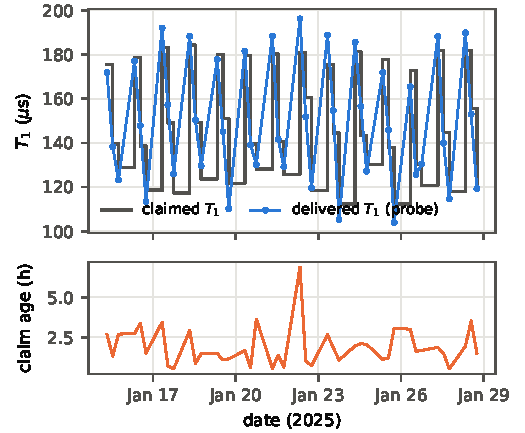
\includegraphics[width=0.93\columnwidth]{F1_concept.pdf}
\caption{The two decoherences on one real device (\texttt{ibm\_brisbane}, 14
days). Top: probe-measured $T_1$ drifts while the claimed calibration value goes
stale between refreshes. Bottom: the age of the claim, the evidence whose decay
LTN models. Claim-versus-probe discrepancy correlates with claim age ($r = 0.34$,
$n = 42$, 95\% CI $[0.04, 0.58]$).}\label{fig:concept}\end{figure}

\begin{figure*}[t]\centering
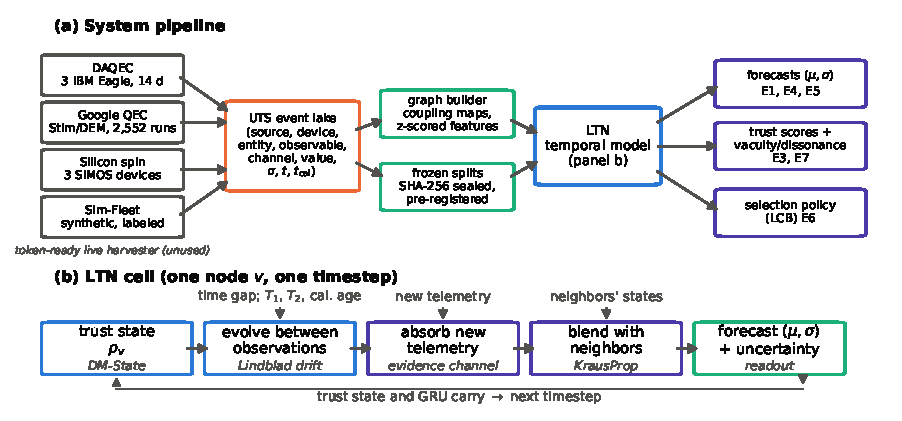
\includegraphics[width=0.78\textwidth]{F2_architecture.pdf}
\caption{System overview. (a)~End-to-end pipeline: four public telemetry sources
(plus a token-ready live harvester, unused here) are normalized into the universal
telemetry event lake, converted by the graph builder into per-device temporal
graphs under SHA-256-sealed pre-registered splits, and consumed by the LTN temporal
model, whose outputs feed the three experiment families (forecasting, trust
semantics, selection). (b)~One LTN cell for node $v$ at one timestep: the trust
state evolves over the time since the last observation, at rates set by the device's
$T_1$, $T_2$ and calibration age; absorbs the new telemetry; blends with its graph
neighbors' states; and is read out as trust scores, a Gaussian forecast, and the
entropy, vacuity and dissonance summaries. The state and a GRU carry pass to the next
timestep. Italics name each stage's module (\S\ref{sec:framework}), whose validity
guarantee is enforced by the accompanying unit tests.}
\label{fig:arch}\end{figure*}

% ======================================================================
\section{Related Work}\label{sec:related}

\textbf{Trust evaluation on graphs.} Graph neural trust models such as
TrustGNN~\cite{trustgnn2022}, EvolveTrust~\cite{evolvetrust2026},
DLGTrust~\cite{dlgtrust2025}, and the dynamic, uncertainty-aware
DGTEN~\cite{dgten2025} operate on social or Bitcoin transaction graphs with
real-vector or Gaussian node states and generic learned dynamics (DGTEN, closest to
our setting, uses Gaussian node states with ODE-based residual updates). None
addresses physical infrastructure, none has a physics-informed evolution law, and
none represents evidence through quantum channels. LTN shares DGTEN's dynamic,
uncertainty-aware framing but moves to a new state space (density matrices), a new
dynamics law (learned Lindbladians), and a new domain (quantum hardware telemetry).
E8 evaluates the DM-state on Bitcoin-OTC and Bitcoin-Alpha~\cite{kumar2016bitcoinotc} against an
equal-parameter vector control to show the representation is not domain-bound; it is
an internal architecture ablation, not a re-benchmarking of DGTEN.

\textbf{Quantum graph neural networks.} The QGNN literature quantizes the
\emph{model}, using parameterized quantum circuits as layers, to process classical
data. LTN occupies the inverse, previously empty quadrant: a classical model with a
quantum-structured \emph{representation}, applied to quantum-\emph{generated} data.
No quantum computation is claimed or required (\S\ref{sec:limitations}).

\textbf{Drift characterization and digital twins.} Calibration-drift studies and
digital-twin models \cite{digitaltwin2026}, \cite{daqec2025} forecast single-device
parameters with generic ML; they carry no graph structure, no trust semantics, no
claim-versus-delivery distinction, and no cross-platform transfer. LTN subsumes their
forecasting task (E1) and adds the trust layer they lack (E3, E6, E7).

\textbf{Trusted nodes in QKD and verification.} QKD network security models treat
relay trust as a static Boolean or consume labels without learning
\cite{qkdbft2025}; cryptographic verification of quantum clouds is per-job and
complementary, because a continuous trust layer can budget expensive verification
toward low-trust targets, which we leave to future work.

To our knowledge, no prior work combines physics-coupled learned open-system
dynamics over a temporal device graph, training on multi-platform real telemetry,
and calibrated claim-versus-delivery trust semantics.

% ======================================================================
\section{The LTN Framework}\label{sec:framework}

LTN maintains, for every node $v$ of a temporal device graph (qubits, couplers,
qubit subsets, or whole devices), a \emph{trust state}: a density matrix
$\rho_v \in \mathbb{C}^{d\times d}$, $\rho_v \succeq 0$, $\tr\rho_v = 1$ (default
$d{=}4$). The maximally mixed state $\rho = I/d$ is the vacuous prior of total
ignorance, and every operation below maps valid states to valid states by
construction, a property we unit-test rather than assume.

\subsection{Universal telemetry schema}
All five data sources (Table~\ref{tab:data}) are mapped to a single event schema:
$(\text{source},\allowbreak \text{platform},\allowbreak \text{device},\allowbreak
\text{entity},\allowbreak \text{observable},\allowbreak \text{channel},\allowbreak
\text{value},\allowbreak \sigma,\allowbreak t,\allowbreak t_{\mathrm{cal}})$,
where \emph{channel} distinguishes \textsf{claimed} calibration values from
\textsf{probe}-measured and \textsf{delivered} outcomes, giving the
claim-versus-delivery pairing that trust evaluation requires.

\subsection{DM-State}
Node states are parameterized by unconstrained $\theta_v \in \mathbb{R}^{d^2}$ via a
Cholesky factor: $\rho_v = L_vL_v^\dagger / \tr(L_vL_v^\dagger)$ with $L_v$ lower
triangular (positive real diagonal). PSD and unit trace hold for any $\theta_v$, and
gradients flow through the factorization.

\subsection{Lindblad drift: epistemic decoherence}
Between observations, trust states evolve under a \emph{learned} Lindblad master
equation~\cite{lindblad1976}, the same dynamical form that governs the devices'
physical decoherence:
\begin{equation}\label{eq:lindblad}
\dot\rho \;=\; -i[H_v,\rho] \;+\; \sum_{k=1}^{3} \gamma_{v,k}\!
\left( L_k \rho L_k^\dagger - \tfrac{1}{2}\{L_k^\dagger L_k, \rho\} \right),
\end{equation}
with $H_v$ Hermitian from the node embedding and $\{L_k\}$ a shared learned jump
dictionary (initialized to lowering, dephasing, and a cyclic-shift mixing operator).
The physics coupling at the heart of H1 sets the rates,
\begin{equation}\label{eq:gamma}
\gamma_{v,k} \;=\; \mathrm{softplus}\,
g_\theta\!\left(T_1^{(v)}, T_2^{(v)}, \Delta t_{\mathrm{cal}}, \ell_v,
e_{\mathrm{plat}}\right),
\end{equation}
so epistemic decoherence rates are functions of the node's \emph{measured physical}
coherence times and the age of its calibration evidence, with
$\partial\gamma_k/\partial \Delta t_{\mathrm{cal}} > 0$ enforced at initialization:
stale claims decay. Over a gap $\Delta t$ we integrate \eqref{eq:lindblad} in
closed form, vectorizing the generator to a $d^2{\times}d^2$ superoperator (column
stacking, so that $\mathrm{vec}(A\rho B)=(B^\top\!\otimes A)\,\mathrm{vec}(\rho)$)
and applying a batched matrix exponential. The resulting channel is CPTP for any
parameters (trace error $<10^{-8}$, Choi minimum eigenvalue $>-10^{-7}$), and for
general Hermitian $H$ at $d{=}4$ it reproduces an independent \texttt{qutip}
Lindblad integration to $<10^{-9}$; both are checked in the accompanying tests.
At initialization the unital (mixing) dissipators dominate, so evidence-starved
states drift toward the maximally mixed vacuous state: trust decays toward
\emph{ignorance}, never toward unwarranted confidence.

\subsection{Evidence channels and KrausProp}
A telemetry event with features $x \in \mathbb{R}^m$ (per-observable z-scores,
missingness mask, calibration age, platform) updates the state through a learned
CPTP channel: an MLP emits $r{=}4$ matrices $\{A_i\}$, normalized to Kraus operators
$K_i = A_i M^{-1/2}$ with $M = \sum_i A_i^\dagger A_i$, giving
$\rho \leftarrow \sum_i K_i \rho K_i^\dagger$ with $\sum_i K_i^\dagger K_i = I$
exactly. Messages between graph neighbors use the same channel construction
conditioned on edge features (two-qubit gate errors); aggregation is a convex
mixture $\rho_v \leftarrow (1-\beta_v)\rho_v + \beta_v \sum_u \alpha_{uv}\,
m_{u\to v}$ with attention $\alpha_{uv} \propto \exp(\mathrm{Re}\,
\tr(\rho_u\rho_v)/\tau)$. Convexity keeps states valid, and the non-commutativity of
channel composition (Proposition~\ref{thm:fusion}) lives in multi-hop propagation.

\subsection{Readout and uncertainty summaries}
Trust facets are learned POVMs: $E_c = C_c^\dagger C_c$ set-normalized so
$\sum_c E_c = I$; $\mathrm{score}_c = \tr(E_c\rho) \in [0,1]$. Forecasts are
Gaussian $(\mu,\sigma)$ read from the state \emph{after an evidence-free Lindblad
roll to the requested horizon}, so predictive uncertainty inherits the physics of
evidence decay (Fig.~\ref{fig:event}). Overall uncertainty is the von Neumann
entropy $S(\rho)$, the pre-registered E7 signal; we additionally report two
qualitatively distinct, individually
normalized summaries of \emph{why} the state is uncertain: \emph{vacuity}
$v(\rho)=\tfrac{d}{d-1}\,(1-\tr\rho^2)\in[0,1]$, the purity deficit that captures
\emph{absence} of evidence ($v{=}1$ at the maximally mixed state), and
\emph{dissonance}, the off-diagonal coherence mass
$\big(\sum_{i\neq j}|\rho_{ij}|\big)/(d-1)\in[0,1]$ that captures \emph{conflicting}
evidence. These are the density-matrix analogues of the uncertainty and conflict
masses in subjective logic \cite{josang2001logic}; unlike a scalar entropy they
separate the two sources, but they are complementary indicators, not an additive
decomposition of $S(\rho)$: vacuity, like $S(\rho)$, measures mixedness; dissonance is
basis-dependent and can vary at fixed $S(\rho)$.

\subsection{Quantum subjective logic}
Interpreting a density matrix as an agent's degree of belief is the premise of
quantum Bayesianism \cite{qbism2002}; our contribution is not that reading but its
coupling to physics-informed Lindblad trust dynamics. The properties below anchor the
semantics. They are stated under the following assumptions.

\begin{enumerate}
\item[1)] Evidence incorporation and graph propagation act on the trust state by
  completely positive trace-preserving (CPTP) maps.
\item[2)] The \emph{discounting} channel of
  Proposition~\ref{thm:contraction} is unital, $\Phi(I/d)=I/d$. The learned
  dissipators are in general non-unital (e.g.\ the lowering-type $L_0$), so Assumption 2
  restricts that proposition to the discounting sub-class rather than to the full
  trained model.
\item[3)] Within an evidence gap the Lindblad generator is time-local and held
  constant, so propagation over the gap is a one-parameter semigroup.
\item[4)] The forecast head is Gaussian: predictive uncertainty is summarized by
  $(\mu,\sigma)$ rather than by the full predictive law.
\item[5)] Telemetry absent within an injected gap is missing at random with respect
  to the observable being forecast.
\end{enumerate}

\begin{proposition}[Classical embedding]\label{thm:recovery}
Let $\rho=\mathrm{diag}(p_1,\dots,p_d)$. Then (i) the POVM scores reduce to affine
functionals $\mathrm{score}_c=\sum_j (E_c)_{jj}\,p_j$ of $p$ and, by
set-normalization, form a probability vector; (ii) $(\mathrm{score}_c)_c$ and the
vacuity $v(\rho)$ are \emph{not} jointly normalized, but the rescaling
$b_c := (1-v)\,\mathrm{score}_c$, $u := v$, with base rate $a_c := \mathrm{score}_c$,
is a bona fide subjective-logic opinion \cite{josang2001logic} whose projected
probability $b_c + a_c u$ returns $\mathrm{score}_c$; (iii) the correspondence is an
\emph{embedding}, not a bijection, because a diagonal $d$-dimensional state carries $d-1$
free parameters against a multinomial opinion's $2d-1$, so the model realizes a
lower-dimensional family inside the opinion simplex; and (iv) on diagonal states the
evidence channel acts as a column-stochastic (Markov) transition on $p$.
\end{proposition}

\begin{proposition}[Fusion non-commutativity]\label{thm:fusion}
Fusion of two evidence channels is order-independent \emph{if} they admit Kraus
representations $\{K_i\},\{L_j\}$ with $[K_i,L_j]\,P_\rho = 0$ for all $i,j$, where
$P_\rho$ projects onto $\mathrm{supp}(\rho)$. The condition is sufficient but not
necessary.\footnote{Kraus representations are non-unique, and channels may commute as
superoperators with no commuting Kraus pair: the fully depolarizing channel commutes
with every unitary conjugation, yet its Kraus set spans $\mathbb{M}_d$ in every
representation. The representation-independent criterion is commutation of the two
Liouville matrices.}
\end{proposition}

\begin{proposition}[No amplification, unital case]\label{thm:contraction}
Under Assumption 2, a unital discounting channel never \emph{increases} a state's purity:
$\tr\Phi(\rho)^2 \le \tr\rho^2$, so $v(\Phi(\rho)) \ge v(\rho)$ and the discounted
opinion's certainty ($1-$vacuity) cannot exceed the source's.
\end{proposition}

The proofs are given in the Appendix.

Training minimizes $\mathcal{L} = \lambda_1\,\mathrm{NLL}_{\mathrm{Gauss}} +
\lambda_2\,\mathrm{BCE}_{\mathrm{diverge}} + \lambda_3\,\mathrm{recon}_{\mathrm{masked}}
+ \lambda_4\,\mathrm{ECE}_{\mathrm{soft}}$ (Adam, $10^{-3}$ cosine, gradient clip
$1.0$, early stopping on validation CRPS); cross-platform pretraining uses
$\lambda_3$ only (masked-telemetry reconstruction).
$\mathrm{ECE}_{\mathrm{soft}}$ is a differentiable expected-calibration error over
$B{=}15$ bins: writing $w_{ib}$ for the membership of sample $i$ in bin $b$, formed
from sigmoid kernels $\sigma(\kappa(p_i - e_b))$ at the internal bin edges $e_b$ with
sharpness $\kappa{=}50$ and padded so that $\sum_b w_{ib}=1$ exactly,
\begin{equation}
\mathrm{ECE}_{\mathrm{soft}} = \sum_{b=1}^{B} \frac{m_b}{n}\,
  \bigl|\bar{p}_b - \bar{y}_b\bigr|,
\end{equation}
with $m_b = \sum_i w_{ib}$, $\bar{p}_b = \sum_i w_{ib}p_i / m_b$ and
$\bar{y}_b = \sum_i w_{ib}y_i / m_b$. The hard ECE is recovered as
$\kappa \to \infty$; the soft form keeps the term connected to the autograd graph.

% ======================================================================
\section{Experimental Setup}\label{sec:setup}

\textbf{Data (Table~\ref{tab:data}).} All sources are public. \emph{DAQEC}
\cite{daqec2025}: 756 QEC runs on three IBM Eagle devices over 14 days at 8-hour
cadence, pairing claimed calibration ($T_1$, $T_2$, readout, ECR error;
calibration timestamps) with probe-measured values and delivered logical error
rates per qubit subgraph. We use its telemetry columns only, not its authors'
experimental conclusions (\S\ref{sec:limitations}). \emph{Google QEC releases}
\cite{googleqec2024}, \cite{googledynamic2024}, \cite{googlecolor2024}, \cite{googlesycamore2022}: Stim
circuits, detector error models (DEMs), and raw shot data for surface-, color-, and
dynamic-code experiments on Sycamore and Willow; we parse the circuits and shots
with Stim~\cite{stim2021}, extract per-qubit DEM error intensities (calibration
analog), and decode logical error per round with minimum-weight perfect
matching~\cite{pymatching2022} (2{,}552 runs). \emph{Silicon spin qubits}
\cite{tanttu2024silicon}: CZ-fidelity and $T_2$ time series for three SiMOS devices,
including lab-timestamped fidelity traces. \emph{Sim-Fleet} (synthetic, explicitly
labeled): a 16-device, 180-day generative fleet with Ornstein--Uhlenbeck coherence
drift, two-level-system episodes, recalibration renewals, physically coupled gate
and readout errors, claim staleness, and data gaps, fitted to the DAQEC marginals by
least squares. Table~\ref{tab:simval} reports every fitted target statistic, matched
or not, and Fig.~\ref{fig:simval} shows the marginals and the dynamics.

\begin{table}[t]
\centering
\caption{Sim-Fleet validation against DAQEC: every statistic in the fit objective,
reported whether or not it matched. Rel.\ err.\ is (sim $-$ real)/real.
$^{\ddagger}$Sign differs between real and simulated series.}
\label{tab:simval}
\resizebox{\columnwidth}{!}{%
\footnotesize
% AUTO-GENERATED by ltn/sim/validate.py -- do not edit by hand.
% Honest sim-vs-real validation of every fitted target statistic.
% 'Obj.' = the statistic was a term in the least-squares fit objective
% (fit.stat_residual keeps every key finite in both real and sim).
\begin{tabular}{lrrrc}
\toprule
Statistic & Real (DAQEC) & Sim (simfleet-v1) & Rel.\ err. & Obj. \\
\midrule
disc.mean & 0.1037 & 0.1511 & +45.7\% & \checkmark \\
disc.p95 & 0.2836 & 0.3843 & +35.5\% & \checkmark \\
gate\_error\_2q.mean & 0.008017 & 0.005831 & -27.3\% & \checkmark \\
gate\_error\_2q.q10 & 0.00657 & 0.004277 & -34.9\% & \checkmark \\
gate\_error\_2q.q50 & 0.007967 & 0.00569 & -28.6\% & \checkmark \\
gate\_error\_2q.q90 & 0.009627 & 0.007548 & -21.6\% & \checkmark \\
gate\_error\_2q.std & 0.001152 & 0.001349 & +17.1\% & \checkmark \\
readout\_error.mean & 0.01503 & 0.01609 & +7.0\% & \checkmark \\
readout\_error.q10 & 0.0115 & 0.008384 & -27.1\% & \checkmark \\
readout\_error.q50 & 0.01494 & 0.0149 & -0.3\% & \checkmark \\
readout\_error.q90 & 0.01885 & 0.02529 & +34.2\% & \checkmark \\
readout\_error.std & 0.002867 & 0.006999 & +144.1\% & \checkmark \\
recal.mean\_h & 1.313 & 8.324 & +534.0\% & \checkmark \\
t1.acf1$^{\ddagger}$ & -0.156 & 0.2019 & +229.5\% & \checkmark \\
t1.acf3 & 0.4205 & 0.1659 & -60.5\% & \checkmark \\
t1.persist\_mae & 0.06406 & 0.119 & +85.7\% & \checkmark \\
t1\_us.mean & 160.5 & 180.7 & +12.6\% & \checkmark \\
t1\_us.q10 & 120.4 & 90.66 & -24.7\% & \checkmark \\
t1\_us.q50 & 158 & 165.5 & +4.8\% & \checkmark \\
t1\_us.q90 & 204.8 & 288.5 & +40.9\% & \checkmark \\
t1\_us.std & 31.86 & 84.88 & +166.4\% & \checkmark \\
t2\_us.mean & 89.7 & 106.8 & +19.1\% & \checkmark \\
t2\_us.q10 & 68.7 & 65.44 & -4.8\% & \checkmark \\
t2\_us.q50 & 88.49 & 101.5 & +14.7\% & \checkmark \\
t2\_us.q90 & 112.4 & 154.8 & +37.7\% & \checkmark \\
t2\_us.std & 16.87 & 36.5 & +116.4\% & \checkmark \\
\midrule
KS t1\_us & \multicolumn{2}{c}{$D=0.2235$, $p<10^{-16}$} & -- & -- \\
KS t2\_us & \multicolumn{2}{c}{$D=0.2871$, $p<10^{-16}$} & -- & -- \\
KS readout\_error & \multicolumn{2}{c}{$D=0.2078$, $p<10^{-16}$} & -- & -- \\
KS gate\_error\_2q & \multicolumn{2}{c}{$D=0.6546$, $p<10^{-16}$} & -- & -- \\
\bottomrule
\end{tabular}
%
}
\end{table}

\begin{figure}[t]\centering
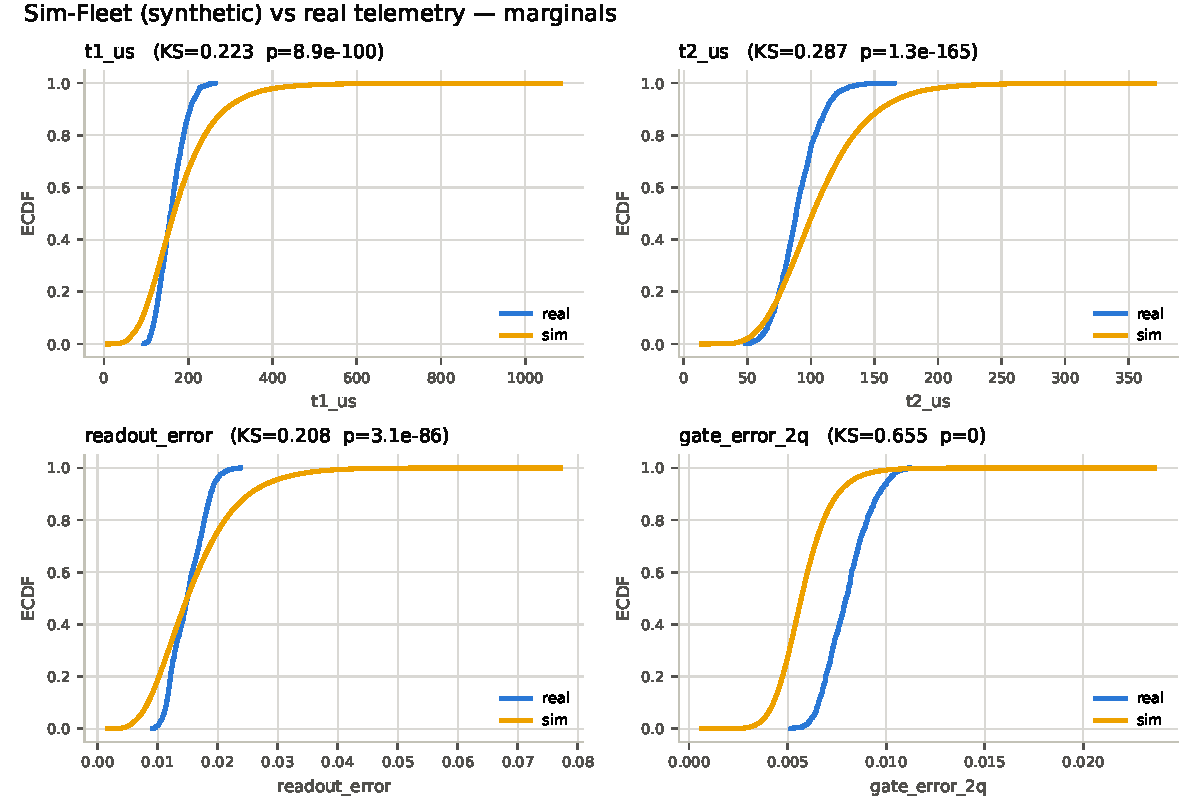
\includegraphics[width=\columnwidth]{simval/sim_vs_real_marginals.pdf}\\[4pt]
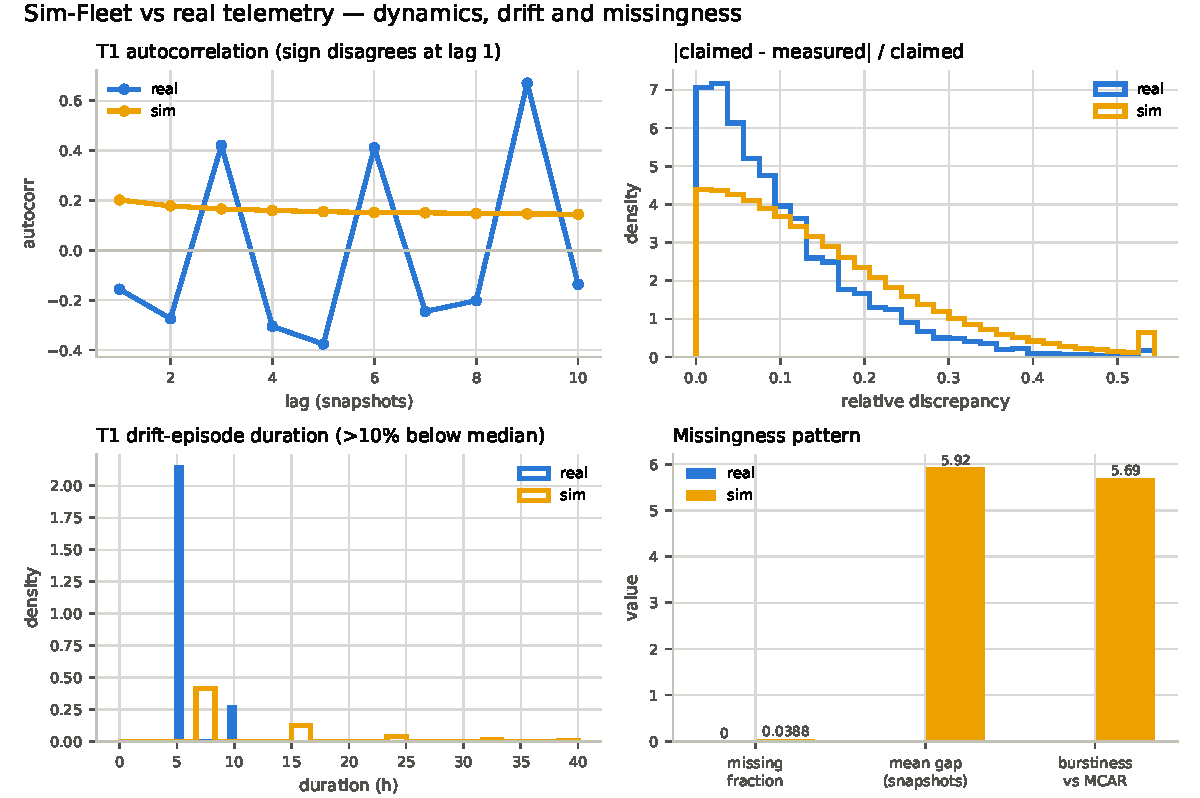
\includegraphics[width=\columnwidth]{simval/sim_vs_real_dynamics.pdf}
\caption{Sim-Fleet vs.\ DAQEC. \emph{Top:} marginal ECDFs. \emph{Bottom:} $T_1$
autocorrelation and claim discrepancy. Statistics are in Table~\ref{tab:simval}.}
\label{fig:simval}\end{figure}

The match is partial, and the misses matter for how Sim-Fleet may be used. The
\emph{static marginals} are reasonable: KS statistics are $0.22$, $0.29$ and $0.21$
on $T_1$, $T_2$ and readout error, with two-qubit gate error matching poorly
(KS $0.65$). The \emph{dynamics} are not. Lag-1 autocorrelation of $T_1$ has the
wrong sign (real $-0.156$, sim $+0.202$): the real series oscillates on a
recalibration-driven cadence that the simulator's monotone decay does not reproduce.
Day-over-day persistence error, which sets forecasting difficulty, is $86\%$ too high
in simulation ($0.064$ real vs.\ $0.119$ sim), and the recalibration renewal interval
is off by a factor of $6.3$ ($1.31$~h real vs.\ $8.32$~h sim). These were all terms
in the fit objective, so they are failures of the fit rather than unfitted extras.
Consequently we treat Sim-Fleet as a stress environment with realistic marginals and
\emph{unrepresentative temporal structure}: it drives E1b and E2 model comparison
(internal validity only), pretraining, E4b, E6a, and E7 gap injection, and no
headline claim rests on it alone. Because the simulated series are both easier to
persist against and more slowly recalibrated than the real ones, sim-only conclusions
about forecasting difficulty and about staleness should not be transported to real
hardware. A post-hoc refit with a recalibration-reset process (\emph{Sim-Fleet-R}) reproduces
these dynamics (lag-1 $-0.20$, persistence error $0.068$, interval $1.40$~h), and E7 is
rerun on it. No live IBM access is used anywhere; the harvester is dry-run-tested and
token-ready.

% \begin{table}[t]\centering
% \caption{Sim-Fleet validation against DAQEC: every statistic in the fit objective,
% reported whether or not it matched. Rel.\ err.\ is (sim $-$ real)/real.
% $^{\ddagger}$Sign differs between real and simulated series.}
% \label{tab:simval}
% \footnotesize
% % AUTO-GENERATED by ltn/sim/validate.py -- do not edit by hand.
% Honest sim-vs-real validation of every fitted target statistic.
% 'Obj.' = the statistic was a term in the least-squares fit objective
% (fit.stat_residual keeps every key finite in both real and sim).
\begin{tabular}{lrrrc}
\toprule
Statistic & Real (DAQEC) & Sim (simfleet-v1) & Rel.\ err. & Obj. \\
\midrule
disc.mean & 0.1037 & 0.1511 & +45.7\% & \checkmark \\
disc.p95 & 0.2836 & 0.3843 & +35.5\% & \checkmark \\
gate\_error\_2q.mean & 0.008017 & 0.005831 & -27.3\% & \checkmark \\
gate\_error\_2q.q10 & 0.00657 & 0.004277 & -34.9\% & \checkmark \\
gate\_error\_2q.q50 & 0.007967 & 0.00569 & -28.6\% & \checkmark \\
gate\_error\_2q.q90 & 0.009627 & 0.007548 & -21.6\% & \checkmark \\
gate\_error\_2q.std & 0.001152 & 0.001349 & +17.1\% & \checkmark \\
readout\_error.mean & 0.01503 & 0.01609 & +7.0\% & \checkmark \\
readout\_error.q10 & 0.0115 & 0.008384 & -27.1\% & \checkmark \\
readout\_error.q50 & 0.01494 & 0.0149 & -0.3\% & \checkmark \\
readout\_error.q90 & 0.01885 & 0.02529 & +34.2\% & \checkmark \\
readout\_error.std & 0.002867 & 0.006999 & +144.1\% & \checkmark \\
recal.mean\_h & 1.313 & 8.324 & +534.0\% & \checkmark \\
t1.acf1$^{\ddagger}$ & -0.156 & 0.2019 & +229.5\% & \checkmark \\
t1.acf3 & 0.4205 & 0.1659 & -60.5\% & \checkmark \\
t1.persist\_mae & 0.06406 & 0.119 & +85.7\% & \checkmark \\
t1\_us.mean & 160.5 & 180.7 & +12.6\% & \checkmark \\
t1\_us.q10 & 120.4 & 90.66 & -24.7\% & \checkmark \\
t1\_us.q50 & 158 & 165.5 & +4.8\% & \checkmark \\
t1\_us.q90 & 204.8 & 288.5 & +40.9\% & \checkmark \\
t1\_us.std & 31.86 & 84.88 & +166.4\% & \checkmark \\
t2\_us.mean & 89.7 & 106.8 & +19.1\% & \checkmark \\
t2\_us.q10 & 68.7 & 65.44 & -4.8\% & \checkmark \\
t2\_us.q50 & 88.49 & 101.5 & +14.7\% & \checkmark \\
t2\_us.q90 & 112.4 & 154.8 & +37.7\% & \checkmark \\
t2\_us.std & 16.87 & 36.5 & +116.4\% & \checkmark \\
\midrule
KS t1\_us & \multicolumn{2}{c}{$D=0.2235$, $p<10^{-16}$} & -- & -- \\
KS t2\_us & \multicolumn{2}{c}{$D=0.2871$, $p<10^{-16}$} & -- & -- \\
KS readout\_error & \multicolumn{2}{c}{$D=0.2078$, $p<10^{-16}$} & -- & -- \\
KS gate\_error\_2q & \multicolumn{2}{c}{$D=0.6546$, $p<10^{-16}$} & -- & -- \\
\bottomrule
\end{tabular}

% \end{table}

\textbf{Pre-registration and splits.} Hypotheses, success bars, kill criteria,
statistical protocol, and tuning budgets were frozen before any experiment run;
deviations are declared inline and in the accompanying deviation register. Splits are
committed with SHA-256
seals: E1a temporal 70/10/20 on DAQEC (horizons 1/3/7 days); E1b temporal on
Sim-Fleet with four held-out devices (1/3/7/14 days); E3 three-fold device
rotation; E4 device holdout; E5 platform holdout (Google never enters training);
E6 replay windows; E8 temporal edge split. Normalization statistics are computed
on training partitions only and stored inside the split files.

\textbf{Baselines and fairness.} Persistence, EWMA, per-series ARIMA, and
LSTM, TGN-style~\cite{tgn2020}, and causal-transformer forecasters share the same
feature sets, split files, and evaluation pairs as LTN\@. Rather than fix capacity and
tune the rest, we gave every learned model an \emph{identical} tuning budget (50
Optuna~\cite{akiba2019optuna} trials, TPE, validation NCRPS objective; persistence
has no hyperparameters) with width/capacity itself a tuned dimension over a
comparable range; the models are therefore \emph{budget-matched}, not
capacity-matched, and the tuned sizes span $17$k to $282$k trainable parameters
(Table~\ref{tab:main}, Params column). Consequently no capacity claim is made in
LTN's favor: on the real split the strongest baseline (LSTM) is in fact several times
\emph{smaller} than LTN, while on the synthetic split the strongest baselines
(TGN, transformer) are several times larger; LTN ties both without being
capacity-privileged. Parameter matching to $\pm10\%$ \emph{is} enforced only for the
E2 ablation variants, which must be capacity-controlled to isolate a module's
contribution. Our scale-free aggregate is NCRPS, defined as the Gaussian
CRPS~\cite{gneiting2007crps} divided by the training standard deviation of the
observable; raw CRPS is reported per cell.

\textbf{Statistics.} Following the journal's convention we write \emph{s-significant}
where we intend the exact statistical sense, at $\alpha=0.05$ ($p<0.05$, or a 95\%
interval that excludes zero). Five seeds per stochastic model (deterministic baselines run
once and are paired against each seed). The unit of analysis is the
device$\times$observable$\times$horizon \emph{cell}: we reduce each cell to its mean
paired CRPS difference and run one Wilcoxon signed-rank test over cells, rather than
testing individual forecast origins. Rolling origins within a series are strongly
dependent (E1b averages $2{,}298$ pairs per cell drawn from a single series), so
treating them as independent inflates the effective sample size (it produces
$p$-values as small as $10^{-133}$). Holm correction controls multiplicity but not
this dependence, which is why the unit, not the correction, is what we changed.
Cliff's $\delta$ gives effect sizes~\cite{cliff1993}; Holm~\cite{holm1979} is retained
for the per-cell breakdowns. Confidence intervals are 10k-resample \emph{cluster}
bootstraps resampling (device, observable) series. We verified the choice of cluster
variable: device-only clustering returns intervals \emph{narrower} than iid for the
deterministic baselines, the small-$k$ degeneracy, so the series is the correct
cluster.

\begin{table*}[t]\centering\caption{Data inventory. SIM rows are synthetic.}
\label{tab:data}
\footnotesize\setlength{\tabcolsep}{3.5pt}
\begin{tabular}{llrrrll}
\toprule
Source & Device & Events & Ent. & Obs. & Span & Type \\
\midrule
sim (16 devices)\textsuperscript{b} & 16 devices & 1,929,938 & 23--247 & 5 & 2026-01-01--2026-06-29 & SIM \\
daqec\textsuperscript{a} & ibm\_brisbane & 4,788 & 4 & 8 & 2025-01-15--2025-01-28 & real \\
daqec\textsuperscript{a} & ibm\_kyoto & 4,788 & 4 & 8 & 2025-01-15--2025-01-28 & real \\
daqec\textsuperscript{a} & ibm\_osaka & 4,788 & 4 & 8 & 2025-01-15--2025-01-28 & real \\
google\_qec & google\_105q & 11,604 & 119 & 3 & 2024-08-01--2024-08-18 & real \\
google\_qec & google\_color & 6,720 & 29 & 3 & 2024-12-01--2024-12-20 & real \\
google\_qec & google\_dynamic & 5,369 & 86 & 3 & 2024-12-01--2024-12-11 & real \\
google\_qec & google\_sycamore\_2022 & 2,079 & 30 & 3 & 2022-07-01--2022-07-06 & real \\
silicon & simos\_a & 1,257 & 3 & 4 & 2022-06-06--2023-02-18 & real \\
silicon & simos\_b & 2,166 & 3 & 4 & 2022-06-02--2023-05-31 & real \\
silicon & simos\_c & 2,580 & 3 & 4 & 2022-09-01--2023-07-24 & real \\
\bottomrule
\end{tabular}
\\[3pt]{\footnotesize\raggedright \textsuperscript{a}\,DAQEC telemetry columns are
used; the dataset's own experimental conclusions are not relied upon.
\textsuperscript{b}\,The 16 synthetic devices are summarized on one row; the
per-device inventory is in the accompanying artifact. Forecast origins (series
$\times$ origin time; train/val/test): E1a and E2, DAQEC 1,248/576/1,152; E1b and E2,
Sim-Fleet 492,448/119,916/192,612; E3, 168 labeled DAQEC snapshots per held-out device;
E4a, \texttt{ibm\_osaka} adapted on 144--480 and evaluated on 384; E4b, four held-out
Sim-Fleet devices adapted on 5,916--61,171 and evaluated on 69,217; E5, silicon 4,168
for training and DAQEC 1,968 for early stopping. Google contributes none: E5 ranks its
55 subgraphs zero-shot.\par}
\end{table*}

% ======================================================================
\section{Results}\label{sec:results}

\subsection{H1: forecasting device telemetry (E1, E2)}\label{sec:results-h1}

Table~\ref{tab:main} reports NCRPS on the frozen test regions; Fig.~\ref{fig:crps}
resolves horizons. On real DAQEC telemetry (E1a) LTN (0.292) \textbf{does not beat
the baselines}: it is edged by LSTM (0.270) and TGN (0.279), and against the best
baseline (LSTM) it is worse in $91.7\%$ of the 36
device$\times$observable$\times$horizon cells (cell-level Wilcoxon over 36 cells,
$p = 4.3\times10^{-7}$, Cliff's $\delta = 0.162$). Against the classical
ARIMA (0.290) the honest verdict is a tie, not the loss the raw means suggest: the
median Cliff's $\delta$ is $0.076$ (negligible) and LTN wins 15 of the 36 cells. The
$0.002$ gap in the means is also smaller than the seed noise behind it, for reasons
we take up next. On the large synthetic fleet (E1b: per-qubit, 12 training
devices, 126 training days) the four neural models cluster within $0.9\%$
(transformer/LSTM 0.310, TGN 0.311, LTN 0.312); LTN is nominally last among them
but clears the classical floor, and the effect sizes are negligible even where the
tests reject (cell-level Wilcoxon vs.\ the transformer over 240 cells,
$p = 8.7\times10^{-24}$, Cliff's $\delta = 0.022$, LTN worse in $78.8\%$ of cells).

Widening the intervals to respect the series structure changes three comparisons, one
in LTN's favour and two against it. On E1b the paired LTN-versus-TGN difference
($-0.0010$) no longer excludes zero once clusters are resampled ($[-0.0026, +0.0005]$,
against $[-0.0018, -0.0003]$ iid), so a finding against LTN becomes a tie. On E1a,
however, LTN's advantages over the Gaussian-process ($+0.0455$) and Kalman
($+0.0488$) baselines of \S\ref{sec:relbaselines} both cease to exclude zero
($[-0.0106, +0.1076]$ and $[-0.0042, +0.1072]$, against iid intervals that excluded
it), so LTN loses two nominal wins. Every finding that LSTM and the transformer beat
LTN survives. On E1a the clustered marginal intervals of all eight models overlap,
including persistence, so that split does not separate any of the eight pre-registered
arms from one another; it does separate all of them from the monotone-degradation
baselines of \S\ref{sec:relbaselines}. The pre-registered \emph{beats the best baseline} bar for H1 is
therefore \textbf{not met on either split}; on real data LTN is third of the four
learned models. We conclude the physics-structured representation carries no
point-forecasting advantage, and any justification must come from the state
semantics evaluated under H2 and H3.

\textbf{One seed, not one model.} LTN's E1a mean is not a typical run. Its five
seeds are $0.277$, $0.279$, $0.281$, $0.288$ and $0.338$: four cluster inside
$0.012$ while one diverges, and that single seed alone moves the mean from $0.281$
to $0.292$ (robust $z = 10.2$). The effect is not unique to LTN, because the transformer
diverges on one E1a seed too ($0.333$ against a median of $0.294$), but it is
largest for LTN, whose seed standard deviation is $\pm0.026$. We keep the
pre-registered mean as the headline everywhere (over ten seeds, five added post hoc,
it is $0.286$, still third), and flag each conclusion whose \emph{sign} depends on
that seed; the E1b split shows no such instability
($\pm0.003$).

The ablations (Table~\ref{tab:ablations}, Fig.~\ref{fig:ablations}) are exactly
such a case. Taken at face value every E1a ablation is nominally \emph{better} than
the full model, by $0.011$ (neural ODE~\cite{neuralode2018} and $-$graph) down to
$0.006$ ($-$physics-$\gamma$). Every one of those advantages is manufactured by the
diverging seed: comparing seed \emph{medians} instead reverses all four signs, and
the full model then leads by $0.001$ (neural ODE), $0.000$ ($-$graph), $0.004$
($-$Gaussian) and $0.001$ ($-$physics-$\gamma$), negligible in the other
direction. The claim that survives either way is the null one: no ablation
\emph{reproducibly} changes accuracy, and none reproducibly helps. In particular
the exact Lindblad exponential and a parameter-matched neural ODE are
indistinguishable ($0.281$ vs.\ $0.282$ by median), so the Lindblad form buys
nothing over a generic learnable ODE for forecasting, a conclusion the robust
statistics support more cleanly than the means did. A dimension sweep of v1 on E1b
is equally flat: $d\in\{2,4,8\}$ give $0.309/0.309/0.309$, so the Hilbert-space
dimension does not drive accuracy either. A v2 sweep on E1a (\S\ref{sec:v2}) agrees, but
the two differ in model, split and dimensions, so they are consistent rather than
strictly independent replications.

\textbf{Where the variance comes from, and a mechanism we had to withdraw.} The
divergence is attributable to the learned Hamiltonian, but the mechanism we first
proposed for \emph{why} is contradicted by measurement, and we report the retraction
rather than the hypothesis.

The hypothesis was this. Between observations LTN integrates
$\exp(\mathcal{L}_v \Delta t)$ over gaps reaching tens of grid units, and the learned
Hamiltonian enters $\mathcal{L}_v$ through the anti-Hermitian commutator
$-i[H_v,\cdot]$, a purely oscillatory term that contributes no contraction. Nothing
then damps the parameter-sensitivities of the exponential as the gap grows, and the
Hamiltonian is not small once trained: on the E1a drift slice $\|H_v\|_F$ has median
$6.9$, inflating the generator norm from $0.70$ to $19.6$ ($21.8\times$ per
generator). Large argument with no decay is the classic regime for a non-normal
generator to amplify sensitivities.

To test it we captured every Lindblad generator each fitted E1a model actually used
(drift steps and evidence-free horizon rolls, $15{,}120$ Liouvillians in total)
and measured seventeen conditioning diagnostics per seed: Henrici departure from
normality, eigenvector condition number $\kappa_2(V)$, numerical abscissa, spectral
gap, commutator norms, and gradient norms at the fitted parameters.
\textbf{The mechanism fails.} On $16$ of the $17$ diagnostics the diverging seed
ranks fourth or fifth of five, and on all $15$ that measure non-normality it ranks
fourth or fifth. It has the \emph{smallest} Henrici departure ($0.227$ against a
median $2.07$ for the other four), the smallest $\|H_v\|_F$ ($3.76$ vs.\ $8.32$), the
smallest numerical abscissa ($0.022$ vs.\ $0.385$), and the smallest gradient norms
(mean $1.05$ vs.\ $1.23$--$1.88$; maximum $1.57$ vs.\ $2.19$--$4.29$). The single
diagnostic on which it ranks second, the ratio of Hamiltonian to dissipative
content, is topped by seed 4, the \emph{best}-performing run. With five seeds no
correlation could be s-significant ($|\rho_s| \le 0.6$, $p \ge 0.28$ throughout), which
is why the rank of the diverging seed is the readable signal; it points the wrong way.

A second check dissolves the framing as well: the $-$Hamiltonian ablation does not
make the generator normal. v1's jump dictionary is itself non-normal, so zeroing
$H_v$ leaves a \emph{more} non-normal dissipator on all five seeds (relative
departure $0.013$--$0.161$ rises to $0.205$--$0.490$). Only the repaired model of
\S\ref{sec:v2} is actually normal ($\kappa_2(V) = 1.000000$ exactly). The ablation
therefore isolates \emph{$H_v$ present versus absent}, not \emph{non-normal versus normal}.

We state the limit of this evidence. These are properties of the fitted parameters;
no per-epoch checkpoints were retained, so a transient instability during training
cannot be inspected retrospectively. That cuts both ways, because the original mechanism
was also a claim about a trajectory we never measured, but every quantity we can
measure points away from it. The causal attribution below stands on its own and does
not depend on the mechanism.

The $-$Hamiltonian ablation
(Table~\ref{tab:ablations}) holds the tuned configuration, the parameter count and
every other module fixed, and only zeroes $H_v$ in the generator; because it reuses
the same seeds, it supports a \emph{paired} comparison that a variance ratio cannot.
The result is unambiguous. Seed 3, the diverging run, moves $0.338 \to 0.274$ when
$H_v$ is switched off, while the four healthy seeds move by at most $0.007$ and the
median is untouched ($0.2808 \to 0.2809$). The Hamiltonian is what diverges; it is
not what forecasts.

Two cautions keep this honest. First, we make no claim of an s-significant variance
\emph{ratio}: the seed standard deviation drops $\pm0.026 \to \pm0.005$, and to the
repaired model's $\pm0.002$, but no variance test rejects, at five seeds (Levene
$p = 0.38$ and $0.27$, bootstrap ratio CI $[0.9, 59]$) or at ten ($p = 0.44$ and
$0.37$), because none of the new runs diverges. The evidence here is the paired seed
and the disappearance of the divergence ($1/10$ runs to $0/10$), not a $p$-value on
a spread. Second, $-$Hamiltonian
does not reach the repaired model's stability ($\pm0.005$ vs.\ $\pm0.002$), so $H_v$
is the cause of the divergence but not the whole account of the spread; the bounded
clock and the unital dictionary of \S\ref{sec:v2} carry the remainder. The rest of
the ablation set agrees: the two variants that drop $H_v$ as a side effect are the
steadiest of the five ($\pm0.002$ neural ODE, $\pm0.003$ ${\to}$Gaussian) and the two
least stable retain it ($\pm0.026$ full, $\pm0.016$ $-$physics-$\gamma$), with
$-$graph the exception at $\pm0.005$.
We therefore make no forecasting claim for the density-matrix structure; if the
Lindblad form has value it is its interpretable, CPTP-guaranteed semantics, not
accuracy.

\begin{table}[t]\centering\caption{Main forecasting results (NCRPS, lower is
better; equal tuning budgets). Intervals are 95\% \emph{cluster} bootstrap CIs
resampling (device, observable) series rather than individual forecast origins, because
rolling origins within a series are not independent; they are $1.7$--$4.6\times$
wider than the iid intervals. Pre-registered arms are listed first; LTN-v2 is the
post-hoc repaired model of \S\ref{sec:v2}, reported under the same protocol but
separated because it was not pre-registered. It is not a separate baseline, and on
E1a its mean gain comes from removing a diverging seed rather than from better
forecasts.}
\label{tab:main}
\footnotesize\setlength{\tabcolsep}{3.2pt}
\begin{tabular}{lcccr}
\toprule
Model & NCRPS [95\% CI] & Seed med.\ (IQR) & Seeds & Params \\
\midrule
\multicolumn{5}{l}{\emph{E1a (real, DAQEC)}} \\
\textbf{LSTM} & \textbf{0.270 [0.223, 0.319]} & 0.269 (0.006) & 5 & 16,808 \\
TGN & 0.279 [0.231, 0.334] & 0.278 (0.004) & 5 & 208,190 \\
ARIMA & 0.290 [0.231, 0.347] & -- & 1 & -- \\
LTN & 0.292 [0.248, 0.344] & 0.281 (0.010) & 5 & 77,860 \\
Transformer & 0.300 [0.245, 0.357] & 0.294 (0.004) & 5 & 26,144 \\
EWMA & 0.375 [0.287, 0.463] & -- & 1 & -- \\
Persistence & 0.424 [0.312, 0.548] & -- & 1 & -- \\
\midrule
\multicolumn{5}{l}{\emph{post-hoc, not pre-registered}} \\
LTN-v2 (\S\ref{sec:v2}) & 0.280 [0.229, 0.336] & 0.281 (0.002) & 5 & 67,852 \\
\midrule
\multicolumn{5}{l}{\emph{E1b (Sim-Fleet, synthetic)}} \\
\textbf{Transformer} & \textbf{0.310 [0.280, 0.341]} & 0.309 (0.001) & 5 & 259,622 \\
LSTM & 0.310 [0.281, 0.340] & 0.310 ($<$0.001) & 5 & 36,186 \\
TGN & 0.311 [0.282, 0.343] & 0.311 (0.001) & 5 & 282,196 \\
LTN & 0.312 [0.283, 0.344] & 0.314 (0.004) & 5 & 79,616 \\
ARIMA & 0.319 [0.289, 0.353] & -- & 1 & -- \\
EWMA & 0.329 [0.298, 0.362] & -- & 1 & -- \\
Persistence & 0.431 [0.390, 0.474] & -- & 1 & -- \\
\midrule
\multicolumn{5}{l}{\emph{post-hoc, not pre-registered}} \\
LTN-v2 (\S\ref{sec:v2}) & 0.313 [0.285, 0.344] & 0.313 (0.002) & 5 & 89,138 \\
\bottomrule
\end{tabular}
\end{table}

\begin{figure}[t]\centering
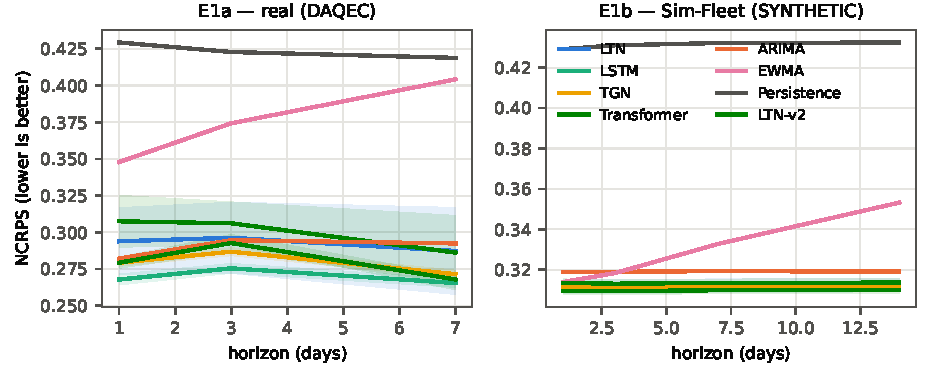
\includegraphics[width=\columnwidth]{F3_crps.pdf}
\caption{NCRPS vs.\ horizon on real (E1a) and synthetic (E1b) telemetry.}
\label{fig:crps}\end{figure}

\begin{table*}[t]\centering\caption{Module ablations (E2), NCRPS (seed means, as
pre-registered, except the $-$Hamiltonian row, which is a post-hoc controlled
ablation added after the variance failure was observed; $\sigma_{\mathrm{seed}}$ is the spread over 5 seeds). Every E1a
ablation is nominally better than the full model, but each advantage is an artifact
of one diverging LTN seed: on seed medians ($\Delta_{\mathrm{med}}$) all four signs
reverse and the full model leads by $\leq0.004$. No ablation reproducibly changes
accuracy in either direction. $-$Hamiltonian is the controlled test of the variance
diagnosis (\S\ref{sec:results-h1}): zeroing $H_v$ alone leaves the median untouched
($0.281$) while the diverging seed recovers, $0.338 \to 0.274$.}
\label{tab:ablations}
\footnotesize\setlength{\tabcolsep}{3.5pt}
\begin{tabular}{lcccccc|cccc}
\toprule
 & \multicolumn{6}{c|}{E1a (real)} & \multicolumn{4}{c}{E1b (sim)} \\
Variant & NCRPS & Med. & IQR & $\Delta$ & $\Delta_{\mathrm{med}}$ & $\sigma_{\mathrm{seed}}$ & NCRPS & Med. & IQR & $\Delta$ \\
\midrule
LTN (full) & 0.292 & 0.281 & 0.010 & -- & -- & 0.026 & 0.313 & 0.313 & 0.003 & -- \\
$-$Lindblad $\to$ neural ODE & 0.281 & 0.282 & 0.003 & $-0.011$ & $+0.001$ & 0.002 & 0.311 & 0.312 & 0.004 & $-0.001$ \\
$-$physics-$\gamma$ & 0.287 & 0.282 & 0.005 & $-0.006$ & $+0.001$ & 0.016 & 0.310 & 0.309 & 0.002 & $-0.003$ \\
$-$DM $\to$ Gaussian state & 0.285 & 0.285 & 0.001 & $-0.007$ & $+0.004$ & 0.003 & 0.311 & 0.310 & 0.001 & $-0.002$ \\
$-$graph & 0.282 & 0.281 & 0.006 & $-0.011$ & $+0.000$ & 0.005 & 0.310 & 0.310 & 0.002 & $-0.002$ \\
$-$Hamiltonian & 0.281 & 0.281 & 0.006 & $-0.012$ & $+0.000$ & 0.005 & -- & -- & -- & -- \\
\bottomrule
\end{tabular}
\end{table*}

\begin{figure}[t]\centering
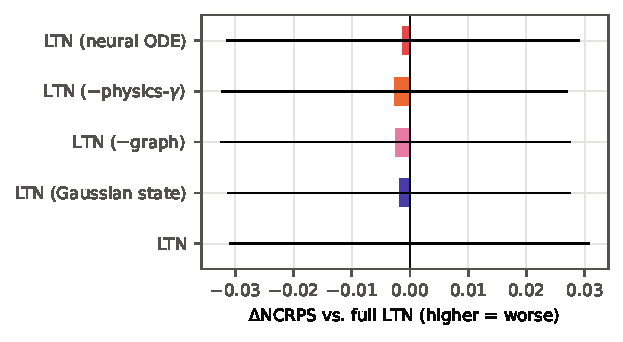
\includegraphics[width=\columnwidth]{F4_ablations.pdf}
\caption{Ablation deltas vs.\ full LTN (E1b, bootstrap CIs).}
\label{fig:ablations}\end{figure}

\subsection{Computational cost}\label{sec:cost}
The measurements in this subsection are \emph{post-hoc}; they were not pre-registered.
The representation is expensive, and because it does not buy accuracy the cost belongs
in the record. Training times are recovered from the campaign's own run records
rather than re-measured; inference figures are medians over $100$ repeats after
warmup on one NVIDIA L40S.

\emph{Training.} On real telemetry (E1a) LTN takes a median $138$\,s against LSTM's
$11.3$\,s, a factor of $12$; LTN-v2 takes $182$\,s. On the synthetic fleet (E1b) LTN
takes $878$\,s against LSTM's $225$\,s, a factor of $3.9$, and LTN-v2 takes
$4{,}538$\,s, a factor of $20$.

\emph{Inference.} On the E1b workload ($121$ entities, $384$ edges) one forecasting
step costs LTN $5.64$\,ms on GPU against LSTM's $0.14$\,ms and TGN's $0.37$\,ms, and
peak memory is $412$\,MiB against $9.6$\,MiB and $13.4$\,MiB. LTN is therefore
roughly $40\times$ slower and $43\times$ larger in memory than the baseline that
outperforms it.

\emph{Scaling in $d$.} The propagator builds a $d^2\!\times\!d^2$ superoperator and
exponentiates it, so cost grows as $O(d^6)$ per node in time and $O(d^4)$ in memory.
We did not characterize the empirical exponent, and we do not claim one. The
analytic rate alone is enough for the design conclusion, because it would be a
serious constraint only if accuracy improved with $d$: \S\ref{sec:v2} finds NCRPS
flat across $d\in\{4,5,8\}$, and \S\ref{sec:carry} finds the forecast largely
bypasses the state. The density-matrix propagator is thus the most expensive
component of the model, scales worst in the one parameter that governs the trust
state's expressiveness, and is the component the evidence says contributes least.

\subsection{Comparison against classical reliability
models}\label{sec:relbaselines}
Persistence, EWMA and ARIMA are standard forecasting controls but they do not
represent the reliability and degradation literature. We therefore added five
classical reliability models, each fitted per series and each given the same
$50$-trial Optuna budget as every other baseline, running through the identical
evaluation path on the same frozen splits (Table~\ref{tab:relbaselines}). These
models are \emph{post-hoc}; they were not pre-registered.

On real telemetry the two state-space and kernel methods are competitive: a
Gaussian-process degradation model reaches NCRPS $0.338$ and a local-trend Kalman
filter $0.341$, against LTN's $0.292$ and LSTM's $0.270$, placing them between the
transformer ($0.300$) and EWMA ($0.375$). We do not read that mean ordering as a win.
Under the cell-level test we apply everywhere else, LTN separates from neither
($p = 0.19$ against the Gaussian process, $p = 0.13$ against the Kalman filter), and
LTN is the better model in only $17$ of $36$ cells in each case: the mean gap is
carried by a minority of high-error cells, not by a consistent advantage. The three remaining
families do considerably worse (switching state-space $0.512$, Wiener $0.541$,
gamma-process $0.582$), and LTN does separate from all three under the same test
($p < 10^{-9}$ in each case, better in $94$--$97\%$ of cells). For the two
degradation models the reason is structural rather than a tuning failure: Wiener and
gamma processes assume a monotone degradation path, whereas recalibration repeatedly
resets this telemetry, so the monotonicity assumption is violated by construction. We
have no equally specific explanation for the switching state-space result and do not
offer one. We report them because a reliability audience will ask, and
because a model failing for a stated structural reason is more informative than its
omission.

The defensible summary is narrower than a win. LTN separates cleanly from the three
structurally misspecified families, is statistically indistinguishable from the two
well-specified ones, and is itself beaten by the generic recurrent baselines. Nothing
here implicates the density matrix either way, because \S\ref{sec:carry} shows the
forecast largely bypasses the state.

We report this comparison on the real split only. These models are fitted
independently per series, so the cost of an equal $50$-trial tuning budget grows with
the number of series, and the synthetic fleet has two orders of magnitude more of them
than DAQEC\@. We consider the real split the more informative one for a reliability
audience in any case, and we prefer a complete comparison on real telemetry to a
budget-starved one on both.

\emph{Change-point detection (E3; post-hoc).} Drift detectors are not forecasters, because they emit
an anomaly score rather than a predictive distribution, so they belong on E3's
divergence-anticipation task rather than in the NCRPS table. Under the identical fold
rotation, labels and threshold, a causal CUSUM reaches $0.461$ mean AUROC and a causal
Page--Hinkley detector $0.579$; an \emph{offline} binary segmentation, which sees the
whole series and is therefore an optimistic bound rather than a peer, reaches $0.547$.
All are far below the pre-registered $0.75$ bar, and Page--Hinkley merely matches the
trivial last-discrepancy carry-forward ($0.58$). Methods purpose-built for detecting
change also fail here. That strengthens rather than weakens the conclusion in
\S\ref{sec:results-h3}: at this recalibration cadence the divergence signal is absent
for every method we tried, not merely absent for ours.

\begin{table}[t]\centering
\caption{Classical reliability and degradation baselines on real telemetry (E1a),
added post-hoc. Each is fitted per series with the same
$50$-trial tuning budget as every other baseline. Pre-registered arms are listed
first, for reference. Wiener and gamma models assume monotone degradation, which recalibration
violates.}
\label{tab:relbaselines}
\footnotesize
\begin{tabular}{llc}
\toprule
Model & Family & NCRPS \\
\midrule
\multicolumn{3}{l}{\emph{pre-registered (repeated from Table~\ref{tab:main})}} \\
LSTM & recurrent & \textbf{0.270} \\
TGN & temporal graph & 0.279 \\
ARIMA & classical statistical & 0.290 \\
LTN & density-matrix state & 0.292 \\
Transformer & attention & 0.300 \\
EWMA & smoothing & 0.375 \\
Persistence & trivial & 0.424 \\
\midrule
\multicolumn{3}{l}{\emph{post-hoc, not pre-registered}} \\
Gaussian process & GP degradation & 0.338 \\
Kalman (local trend) & linear-Gaussian state space & 0.341 \\
Switching state space & hidden Markov & 0.512 \\
Wiener process & degradation (monotone) & 0.541 \\
Gamma process & degradation (monotone) & 0.582 \\
\bottomrule
\end{tabular}
\end{table}

\subsection{H2: transfer (E4, E5)}\label{sec:results-h2}

Cold start on a held-out real device (E4a, \texttt{ibm\_osaka};
Fig.~\ref{fig:transfer} left): with sim-pretraining and fine-tuning on the two
peer devices, LTN adapted on \textbf{one day} of target-device data reaches NCRPS
$0.360$ (95\% CI $[0.304, 0.417]$), below the $0.545$ ($[0.469, 0.628]$) that a
from-scratch model reaches at \textbf{seven days}. The paired contrast is $0.186$
NCRPS (95\% CI $[0.063, 0.319]$, cluster bootstrap over the 12
observable$\times$horizon series; positive on all five seeds). This is a
$\geq7\times$ data-efficiency gain against the pre-registered $\geq 2.3\times$
bar, and even the zero-shot pretrained model (0.515) beats scratch at any tested
$k$. We state the interval rather than the point estimate because its lower end is a
third of the point contrast: the direction is secure, the magnitude is not. On the synthetic fleet (E4b, four held-out devices) the effect saturates:
pretrained zero-shot (0.309) already beats scratch with 30 days of target
data (0.526), clearing the pre-registered $\geq 4\times$ bar. Because
sim-to-sim transfer shares the generative process, however, E4a is the binding
evidence. As pre-registered this is the paper's one positive result; the post-hoc
baseline comparison below reassigns it from the architecture to pretraining.

\emph{Scope of E4.} Both arms are LTN: as pre-registered, E4 varies
\emph{initialization}, not architecture. It therefore establishes that pretraining
transfers for this model, not that the density-matrix state is what transfers. To find
out which, we ran the identical pretrain-and-fine-tune protocol for the sequence
baselines. The result removes the claim, and we report it in
\S\ref{sec:transfer-baselines}.

\textbf{Do the baselines transfer as well? (post-hoc)}\label{sec:transfer-baselines}
E4 as pre-registered cannot separate \emph{pretraining works} from \emph{the density-matrix
state transfers}. We therefore ran the identical protocol, with the same pretraining
corpus, same masked-reconstruction objective, same tuning budget, same fine-tuning
schedule and adaptation budgets, for LSTM, TGN, and a causal transformer
(Table~\ref{tab:transfer}). Every family uses the five seeds of the E4a run
reported above, so the LTN rows there are that run and the comparison is
seed-matched. All four families run at the same E4 default
hyper-parameters; we did not additionally sweep per-family tuned architectures, so the
baselines are, if anything, handicapped relative to their own optima. This experiment
is post-hoc; it was not pre-registered.

\textbf{The claim does not survive.} Pretraining helps every family, and it helps LTN
\emph{least}: at $k{=}0$ the LSTM improves $0.621 \to 0.434$, TGN $0.604 \to 0.380$
and the transformer $0.596 \to 0.384$, against LTN's $0.581 \to 0.515$. Pretrained LTN
is last of the four families at every adaptation budget tested ($k{=}0$, $1$, $3$,
and $7$ days), with the mean paired difference favouring the baseline in all twelve
(baseline, $k$) cells, though $0$--$1$ of the $5$ seeds favour LTN within each cell.
With five seeds no individual comparison is s-significant ($p \ge 0.0625$, the minimum
attainable at $n{=}5$, reached in five cells), so what we claim is that LTN is never ahead on average, not
that it is s-significantly behind.

The $\geq 7\times$ figure is likewise an artifact of its reference arm. It divides the
target data that \emph{LTN-from-scratch} needs by what pretrained LTN needs, and
LTN-from-scratch does not improve between one and seven days ($0.546$, $0.546$ and $0.545$).
This suggests an under-optimized arm at these small adaptation budgets rather
than a genuinely data-hungry model. A competitive reference changes the picture: the
plain causal transformer, trained from scratch with no pretraining at all, reaches
$0.346$ on one day, which already beats pretrained LTN on one day ($0.360$).
Recomputing the efficiency ratio against the best from-scratch arm anywhere in the
table (that transformer at $0.339$, reached with seven days), pretrained LTN never
matches it (its best is $0.349$), so against this reference it misses the
pre-registered $\geq 2.3\times$ bar, while pretrained LSTM needs three days
($2.3\times$) and TGN and the transformer one ($7.0\times$). Every family clears the original bar
zero-shot.

We therefore withdraw the transfer result as evidence for the density-matrix
representation. What survives is narrower and belongs to the pretraining corpus, not
to the architecture: cross-platform masked pretraining on synthetic and peer-device
telemetry substantially improves cold-start forecasting for \emph{every} temporal
model we tested, and least for ours.

\begin{table}[t]\centering
\caption{Cold-start transfer under an identical pretrain-and-fine-tune protocol
(E4a, real, \texttt{ibm\_osaka} held out; post-hoc, not pre-registered). Mean NCRPS
over 5 seeds, median in parentheses (IQR at most 0.066), lower is better; $k$ is days
of target-device data. Pretrained LTN is last of the four families at every $k$.}
\label{tab:transfer}
\footnotesize\setlength{\tabcolsep}{2.5pt}
\resizebox{\columnwidth}{!}{%
\begin{tabular}{llcccc}
\toprule
Family & Arm & $k{=}0$ & $k{=}1$ & $k{=}3$ & $k{=}7$ \\
\midrule
\multirow{2}{*}{LTN}
 & pretrained & 0.515\,{\scriptsize(0.523)} & 0.360\,{\scriptsize(0.353)} & 0.349\,{\scriptsize(0.338)} & 0.351\,{\scriptsize(0.343)} \\
 & scratch    & 0.581\,{\scriptsize(0.572)} & 0.546\,{\scriptsize(0.534)} & 0.546\,{\scriptsize(0.534)} & 0.545\,{\scriptsize(0.534)} \\
\multirow{2}{*}{LSTM}
 & pretrained & 0.434\,{\scriptsize(0.452)} & 0.342\,{\scriptsize(0.334)} & 0.328\,{\scriptsize(0.324)} & 0.328\,{\scriptsize(0.320)} \\
 & scratch    & 0.621\,{\scriptsize(0.622)} & 0.574\,{\scriptsize(0.570)} & 0.574\,{\scriptsize(0.570)} & 0.573\,{\scriptsize(0.569)} \\
\multirow{2}{*}{TGN}
 & pretrained & \textbf{0.380}\,{\scriptsize(0.360)} & 0.326\,{\scriptsize(0.329)} & 0.313\,{\scriptsize(0.313)} & 0.312\,{\scriptsize(0.312)} \\
 & scratch    & 0.604\,{\scriptsize(0.614)} & 0.522\,{\scriptsize(0.520)} & 0.523\,{\scriptsize(0.522)} & 0.523\,{\scriptsize(0.521)} \\
\multirow{2}{*}{Transformer}
 & pretrained & 0.384\,{\scriptsize(0.367)} & \textbf{0.313}\,{\scriptsize(0.310)} & \textbf{0.299}\,{\scriptsize(0.297)} & \textbf{0.297}\,{\scriptsize(0.292)} \\
 & scratch    & 0.596\,{\scriptsize(0.586)} & 0.346\,{\scriptsize(0.349)} & 0.344\,{\scriptsize(0.343)} & 0.339\,{\scriptsize(0.338)} \\
\bottomrule
\end{tabular}}
\end{table}

\textbf{Zero-shot platform ranking (E5): pre-registered demotion.} Training on
silicon, with IBM telemetry for early stopping, and ranking Google code placements by
predicted error against
decoded logical error per round yields pooled Spearman $\rho = 0.08$--$0.14$
across seeds (permutation $p \geq 0.29$, $n = 55$ subgraphs), below the
pre-registered $\rho < 0.2$ demotion threshold. LTN's learned state is on par with
the raw-DEM-intensity control ($\rho = 0.077$), and neither is s-significant. With the
observable vocabularies this heterogeneous, cross-platform reliability transfer
is \emph{few-shot}, not zero-shot, and H2 rests on E4.

\begin{figure}[t]\centering
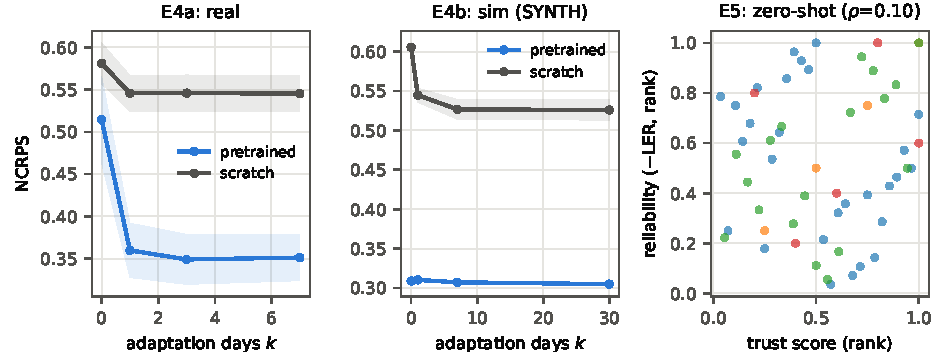
\includegraphics[width=\columnwidth]{F5_transfer.pdf}
\caption{Cold start (E4) and zero-shot platform ranking (E5).}
\label{fig:transfer}\end{figure}

\subsection{H3: trust semantics (E3, E6, E7)}\label{sec:results-h3}

\textbf{Claim-divergence prediction (E3): pre-registered kill, reported.} At
DAQEC's near-continuous recalibration cadence (median per-run claim age $6.5$\,h,
IQR $3.5$--$9.3$\,h, max $12.0$\,h; the freshest calibration available at any snapshot
is a median $2.0$\,h old, IQR $1.2$--$2.9$\,h), relative claim-versus-probe divergence
events are temporally indistinguishable from white noise, because no per-entity lag-1
autocorrelation leaves the white-noise band $\pm 1.96/\sqrt{42} = \pm 0.30$ (event
indicator $\max|r_1| = 0.28$, median $0.13$, over the $9$ non-degenerate entity
series; continuous relative discrepancy $\max|r_1| = 0.30$, median $0.10$, over $36$
series, each with $n=42$ snapshots), and \emph{no} predictor exceeds chance on the
held-out device: LTN dissonance reaches 0.497 AUROC, an LTN state probe 0.511, and a
staleness control 0.459. The best signal anywhere is a trivial last-discrepancy
carry-forward at 0.58, still far below the pre-registered 0.75 bar. We conclude
the divergence-anticipation claim is \textbf{untestable in this regime}: when
claims are refreshed faster than the drift timescale, divergence is measurement
noise. The claim would need telemetry with longer claim-aging (the situation our
gap studies emulate) and we drop it here per the pre-registered kill criterion.

\textbf{Operational value (E6).} A policy selects, at each replay step, a
$w$-qubit subgraph $S$ on which to run a job; a candidate's realized success
probability under the (hidden) ground-truth error rates is
\begin{equation}\label{eq:jobsuccess}
p(S) = \!\prod_{q\in S}\!(1-e^{\mathrm{ro}}_q)(1-e^{\mathrm{1q}}_q)^{G_1}
       \!\!\prod_{(u,v)\in E(S)}\!\!(1-e^{\mathrm{2q}}_{uv})^{G_2},
\end{equation}
with $G_1{=}10$ single- and $G_2{=}5$ two-qubit gate layers, and $e^{\mathrm{ro}},
e^{\mathrm{1q}}, e^{\mathrm{2q}}$ the readout, one- and two-qubit error rates.
Regret is $\max_{S'}p(S')-p(S_{\text{chosen}})$; policies see only claimed values
or LTN forecasts, never the truth. In the truth-driven synthetic replay (E6a,
Fig.~\ref{fig:regret}) every informed policy cuts regret several-fold
vs.\ random, but \emph{no} pairwise difference between the informed policies
(greedy-claimed, LTN-mean, LTN-LCB) separates at 95\% bootstrap CIs over rounds
(cumulative regret at $w{=}12$: LTN-LCB 0.226 vs.\ greedy
0.257). The pre-registered separation bar is not met: LTN
forecasts convert to selection decisions \emph{on par with} the
calibration-greedy operational standard, not beyond it. Informed policies use a
single trained checkpoint, so E6a isolates policy quality, not seed variance. The
logged-arm DAQEC
replay (declared secondary) is degenerate, because logged arms differ by $<0.1\%$ in
delivered success, so no policy separates there either.

\textbf{Uncertainty quality (E7).} We assess calibration with post-hoc temperature
scaling fitted on validation. Temperature scaling was introduced for classifier
logits \cite{guo2017calibration}; the regression analogue we use rescales the
predictive scale, $\sigma \mapsto t\,\sigma$ with
\begin{equation}
t = \arg\min_{t>0} \sum_i \Bigl[\log(t\sigma_i)
  + \frac{(y_i-\mu_i)^2}{2t^2\sigma_i^2}\Bigr],
\end{equation}
the Gaussian negative log-likelihood on the validation split, optimized over
$\log t \in [-10,10]$ by bounded scalar search. It leaves $\mu$ and hence all
sharpness-free accuracy metrics unchanged. On the synthetic fleet the
forecasts are well calibrated (temperature 1.00, 90\% coverage
0.906; Sim-Fleet-R: $1.00$, $0.902$); on real DAQEC they are systematically
\emph{under-dispersed}
(temperature 1.07, 90\% coverage 0.823 raw,
0.847 after scaling), a residual under-coverage we report
rather than hide and attribute to the 14-day non-stationarity. The gap event study,
run on Sim-Fleet (Fig.~\ref{fig:event}, left), returns a clean negative: during injected telemetry
gaps the empirical forecast error grows monotonically to $+11.4\%$ by the fifth
hidden snapshot, while the state entropy $S(\rho_t)$ stays flat ($|\Delta| \leq
0.6\%$) \emph{and} the predictive $\sigma$ (a declared post-hoc diagnostic) is
equally flat ($|\Delta| \leq 1\%$). On Sim-Fleet-R (post-hoc; \S\ref{sec:setup}; gaps of
\mbox{8--40}~h) the negative repeats: error rises to $+6.6\%$ as entropy falls ($+3.1\%
\to +1.2\%$) and $\sigma$ stays within $0.8\%$. The pre-registered entropy-tracks-error claim
\textbf{fails}, and more broadly the trained model is overconfident under
evidence starvation it never saw in training. Two mechanisms are identifiable, and
both are architectural rather than incidental. First, with a horizon-conditioned
forecast head, uncertainty need not route through the Lindblad state, so gradient
pressure on the physics-coupled rates vanishes, and the training distribution
contains no multi-snapshot all-entity gaps to correct it. Second, and worse than
flatness: nothing constrains the learned jump operators to remain normal, and
training pushes them away from it, so the fitted channel is non-unital and
\emph{purifying}. Rolled forward on E1a, the trained model's mean state entropy
\emph{decreases} down the horizon ($1.23 \to 1.10$ for $h = 1\ldots21$, falling for
the large majority of states): the state does not merely fail to decohere, it
\emph{recoheres} (our term for growing purer without new evidence). The entropy
channel could not have tracked growing error even had the
head been willing to listen. Dissonance is likewise static around
recalibration and divergence events (Fig.~\ref{fig:event}, right), consistent
with E3. Forcing predictive $\sigma$ to be read from the state alone is the
architectural change these results motivate, and \S\ref{sec:v2} carries it out rather
than leaving it to future work: it revives $\sigma$ (which then rises through an
evidence gap where v1's was flat; on Sim-Fleet-R only at gap onset, $+2.5\%$) but not
the entropy signature, because the
evidence channel, not the drift, is what governs the state through a gap.

\begin{figure}[t]\centering
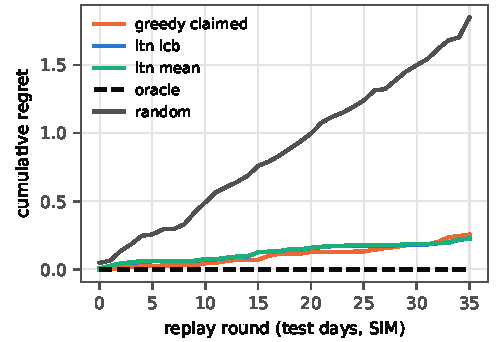
\includegraphics[width=\columnwidth]{F6_regret.pdf}
\caption{Cumulative selection regret under replay (E6a, simulated fleet;
policies see only claimed values or LTN forecasts, outcomes come from hidden
truth).}\label{fig:regret}\end{figure}

\begin{figure*}[t]\centering
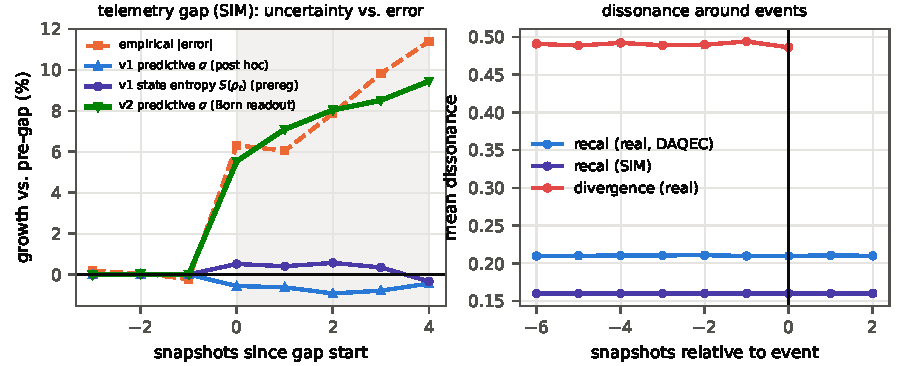
\includegraphics[width=0.71\textwidth]{F7_event.pdf}
\caption{Gap event study on Sim-Fleet. Left: during injected telemetry gaps (shaded)
v1's empirical forecast error grows to $+11.4\%$ while its state entropy $S(\rho_t)$
(pre-registered) and predictive $\sigma$ (post hoc) stay flat; the repaired model's
$\sigma$ (\S\ref{sec:v2}) is the one uncertainty curve that follows the error. Right:
dissonance is static around recalibration and divergence events, consistent with the
E3 null.}
\label{fig:event}\end{figure*}

\subsection{Domain generality (E8)}\label{sec:results-e8}
To test whether the architecture is domain-bound, we drop DM-State and Lindblad decay
into a DGTEN-style pipeline on Bitcoin-OTC and Bitcoin-Alpha (edge-weight prediction
over 40 temporal windows) and compare against an equal-parameter vector-GRU control
in the identical pipeline (Table~\ref{tab:e8}). As in \S\ref{sec:related}, E8 is an
internal architecture ablation, not a re-benchmarking of DGTEN. At the pooled mean the density-matrix
state improves both RMSE and sign-AUROC on both graphs. The two metrics do not,
however, carry equal weight. The RMSE advantage holds on every seed pairing: the worst
LTN seed mean beats the best control seed mean on both graphs. The sign-AUROC
advantage does \emph{not} survive at seed resolution, because the control's seed 4 beats two
LTN seeds on Bitcoin-Alpha and one on Bitcoin-OTC, and that same seed is a large
positive outlier for the control on both graphs, which is equally consistent with the
control being under-trained on its other four seeds. We therefore read E8 as
suggestive evidence on RMSE that the representation is not domain-bound, and we do not
claim the AUROC result. This is the same single-seed pathology we police elsewhere in
the paper, and it deserves the same treatment. Per-observable and per-device result
tables and additional regret widths ($w \in \{5, 27\}$) are provided in the
accompanying artifact.

\begin{table}[t]\centering\caption{Domain generality (E8) on Bitcoin trust graphs:
an internal architecture ablation, not a re-benchmarking of DGTEN.}
\label{tab:e8}
\begin{tabular}{llcc}
\toprule
Dataset & Model & RMSE & sign-AUROC \\
\midrule
Alpha & LTN (DM+Lindblad) & 0.157 & 0.581 \\
Alpha & vector-GRU control & 0.266 & 0.425 \\
OTC & LTN (DM+Lindblad) & 0.174 & 0.628 \\
OTC & vector-GRU control & 0.303 & 0.521 \\
\bottomrule
\end{tabular}
\end{table}

\subsection{Testing the diagnoses: a repaired model}\label{sec:v2}
Two of our negatives came with a mechanism attached: the seed variance was blamed on
the learned Hamiltonian, a causal attribution that survives even though the
non-normality account of \emph{why} does not (\S\ref{sec:results-h1}), and the
failed entropy-growth signature on a readout that lets uncertainty reach the horizon
without passing through the state (\S\ref{sec:results-h3}). A mechanism that cannot
be falsified is not a scientific claim, so we built the model those diagnoses imply
and re-ran the
affected experiments under the same protocol as every other model: the same frozen
splits, the same 50-trial Optuna budget over the same search space, and the same five
seeds for the headline runs (the $d$ sweep uses three per arm, as v1's did; the E1b
tuning completed 49 of its 50 trials after a GPU failure, a shortfall that can only
disadvantage v2).
It changes four things, which is precisely why it can corroborate a diagnosis but
not isolate one.
\emph{(i)~Born-rule readout}: $\mu_c = a_c \tr(\rho_h O_c) + b_c$ and
$\sigma_c = s_c \sqrt{\tr(\rho_h O_c^2) - \tr(\rho_h O_c)^2}$ for learned Hermitian
$O_c$, so $\sigma$ is a functional of the state alone, with no horizon or carry path;
uncertainty can then only grow if the drift mixes the state, which forces
$\partial\sigma/\partial\gamma \neq 0$.
\emph{(ii)~Unital dissipative drift}: $H_v$ is deleted and the jump dictionary is
restricted to Hermitian (hence normal, hence unital) operators. Four properties must
be distinguished here, because only two are theorems. \emph{Unitality} is structural,
holding for any parameters, and \emph{entropy non-decrease} follows from it by
majorization; both hold for any learned rates. \emph{Uniqueness of the fixed point}
does not: it requires the $\{L_k\}$ to generate the full matrix algebra, and Hermitian
dephasing jumps are a standing counterexample, being unital and
entropy-non-decreasing while fixing every diagonal state. For these fits uniqueness
holds \emph{empirically}: the generator's kernel has dimension exactly $1$ in all
$25$ fitted v2 checkpoints, rate-independently (the commutant of $\{L_k\}$ is trivial
in $25/25$), and in all $2{,}520$ generators the model uses on real E1a timelines,
with a rank-determination margin of fourteen orders of magnitude. \emph{Convergence
to $I/d$} then follows, but as an empirical property of these fits, not a guarantee of
the construction. This repairs an \emph{observed} pathology, not a hypothetical one. Nothing in
v1 constrains its jump operators to stay normal, and training drives them away from
it ($\|[L_k,L_k^\dagger]\|$ reaches $0.5$--$1.4$ across the fitted E1a seeds), which makes the
learned channel non-unital and therefore \emph{purifying}. The consequence is a
trust model running in reverse: rolling that model forward, mean state entropy
\emph{falls} along the horizon ($1.23 \to 1.10$ over $h = 1 \ldots 21$, decreasing
for the large majority of states). v1 grows \emph{more} certain the further it
extrapolates from evidence, the exact opposite of the epistemic decoherence the
model is named for, and an anti-signature to the one E7 sought. Restricting to
Hermitian jumps makes the correct direction a structural property rather than
something to hope training respects.
\emph{(iii)~Saturating clock}: the gap enters as
$\tau(\Delta t) = \tau_{\max}(1 - e^{-\Delta t/\tau_{\max}})$, bounding the matrix
exponential's argument; because $\tau$ is concave this is the exact Lindblad
solution in a warped clock, not in physical time.
\emph{(iv)~Observable-aligned state}: $d = n_{\mathrm{obs}}{+}1$.

The variance diagnosis is \textbf{confirmed}. On E1a the repaired model's seed
standard deviation is $\pm0.002$ against $\pm0.026$, no seed diverges (worst run
$0.338 \to 0.282$),
and NCRPS improves to $0.280$: level with TGN (cell-level Wilcoxon over 36 cells,
$p = 0.88$, Cliff's $\delta = -0.04$), still tied with ARIMA but now on the better
side of it, and much nearer LSTM than v1 was. We deliberately do not report this as a
change in rank. None of it is new forecasting skill: against v1's four non-diverging
seeds the difference is $0.280$ vs.\ $0.281$, which no test resolves (seed-level Welch
$p = 0.66$; $0.19$ over ten seeds). The entire movement is the deleted outlier, and a mean over five seeds is
sensitive to one of them. E1b settles
the point. That split never had a diverging seed to repair, and there the repair buys
nothing: v2 and v1 are indistinguishable (median Cliff's $\delta = 0.002$; v2's mean
is $0.001$ higher, last among the learned models). A repair earns nothing where there
is nothing to repair, which is exactly what we should expect and the reason we do not
report it as an improvement. Attribution likewise rests on the controlled $-$Hamiltonian ablation of
\S\ref{sec:results-h1}, not on this model, which moves four things at once and so can
corroborate the diagnosis but never isolate it.

The readout diagnosis is \textbf{confirmed, and the pre-registered signature still
fails}, a split verdict worth stating exactly. We measure it on the same injected
gaps as v1 (Fig.~\ref{fig:event}), tracking each quantity as a percentage of its
pre-gap level so the two models are read the same way. The predictive $\sigma$
finally responds to evidence starvation: through a gap v2's $\sigma$ rises at every
hidden snapshot, from $+5.5\%$ at gap onset to $+9.4\%$ by the fifth, moving with the
empirical error ($+9\%$ to $+11\%$), whereas v1's $\sigma$ drifts slightly \emph{down}
over the same gaps ($-0.6\%$ to $-0.4\%$) and its entropy stays flat. Uncertainty
that could previously ignore the state now cannot, which is precisely what the
Born-rule readout was built to force, and calibration improves with it (real:
temperature $1.07 \to 1.01$, raw 90\% coverage $0.823 \to 0.852$; simulated:
$1.00 \to 0.99$, $0.906 \to 0.908$). Yet the pre-registered claim, that
\emph{entropy} tracks error, fails again, and for a reason the repair exposes rather
than removes. v2's entropy does jump when a gap opens (evidence loss raises it $+12\%$
over the pre-gap level), but it then drifts back \emph{down} as the gap deepens
($+12.2\%$ at onset to $+9.9\%$ at the fifth snapshot) while the error keeps climbing,
so it does not track error. Decomposing one gap step of the trained model shows why:
the unital drift raises entropy for every node (exactly the guarantee), but the
evidence channel, which is CPTP yet not unital and is still applied through a gap because the
snapshot is empty rather than absent, then removes more than the drift added. The
guarantee we bought is real and it binds on the drift; the drift is simply not what
governs the state through a gap. Making evidence unital under a null observation, so
that seeing nothing cannot sharpen a belief, is the change this points to and the one
we have not yet tested. We stop short of claiming $\sigma$ \emph{tracks} error: the
across-position correlation rises from $-0.24$ to $+0.81$, but with six gap depths it
is not resolvable from zero, and the empirical error is itself noisy. What is
established is narrower and still worth having: the uncertainty channel is now
connected to the state.

The representation diagnosis \textbf{does not survive}. If the density matrix were
doing the forecasting once $\sigma$ is forced through it, accuracy would have to
respond to its dimension. It does not: on E1a, $d\in\{4,5,8\}$ (3 seeds each) give
$0.279/0.279/0.280$, a spread of $0.0005$ that is $0.22\times$ the within-$d$ seed
noise. We read this as equivalence rather than as a large $p$: the whole effect of
doubling $d$ is bounded well inside the noise of re-running the same $d$, which is
the practical definition of not mattering. It echoes v1's flat sweep
($0.309/0.309/0.309$), though that one varied $d\in\{2,4,8\}$ on the synthetic
split, so the two are consistent rather than strictly independent replications.
The repaired model is therefore not a better forecaster, and we do not present it as
one. Its value is negative evidence made sharper, and it defines what would have to
change for a physics-structured state to earn its place: a task where the state, not
the recurrent carry, is the thing being asked for.

\subsection{Reliability endpoints}\label{sec:reliability}
These endpoints are \emph{post-hoc}; they were not pre-registered, and they re-score
the pre-registered forecasts rather than adding new model runs. NCRPS measures
forecast quality, not reliability. Because the forecasts are Gaussian,
three reliability quantities follow in closed form from the stored $(\mu,\sigma)$
without retraining or refitting, so they cannot flatter any model relative to the
numbers already reported (Table~\ref{tab:reliability}).

\emph{SLA-violation probability.} Writing $q$ for a per-device, per-observable
specification limit, $P(Q_{t+h}\ \text{out of spec}) = \Phi((\mu-q)/\sigma)$ for error
rates and $\Phi((q-\mu)/\sigma)$ for coherence times. We set $q$ at the empirical
quantile of the observed outcomes that puts $10\%$ of mass out of spec, computed from
$y$ alone so it is identical for every model; LTN remains mid-pack and behind both the transformer and LSTM at
$5\%$, $10\%$ and $20\%$, though the ordering among the other arms shifts (ARIMA in
particular falls from first to fifth as the threshold loosens). On the synthetic fleet LTN is mid-pack: a paired device-clustered
bootstrap puts it s-significantly \emph{worse} than the transformer
($+0.00063$, $[+0.00035, +0.00114]$) and LSTM ($+0.00062$, $[+0.00007, +0.00171]$),
indistinguishable from TGN, ARIMA and LTN-v2, and better only than EWMA and
persistence. The reliability endpoint therefore reproduces the H1 verdict rather than
overturning it, which is the outcome we would expect if the two measure the same
underlying forecast quality.

\emph{Reliability function and hazard.} Chaining $(1-p_{\mathrm{viol}})$ across
checkpoints gives $R(h)$; LTN's chained survival is mildly pessimistic at the longest
horizon ($\Delta R(14) = -0.006$, against $-0.001$ for the transformer and $-0.113$,
$-0.128$ for EWMA and persistence). We caution against a physical reading of the
declining per-checkpoint hazard ($0.102 \to 0.048$ from $h{=}1$ to $h{=}14$): the
checkpoint spacing widens over the same range, and the surviving cohort is
disproportionately the stable device--observable pairs, so this is frailty, not a
decreasing failure rate.

\emph{Expected wasted shots and availability.} On the synthetic replay, with $4096$
shots per job, informed selection recovers roughly $220$ shots per job against random
at width $12$, a large and robust effect. Informed policies do not separate from one
another: LTN-LCB leads greedy-claimed at widths $5$ and $12$ but trails it at width
$27$, and all three lie within $\sim14$ shots of one another, out of $4096$. This matches the E6 regret
null and we claim no separation. On the real logged replay the lane is degenerate:
random selection wastes $0.51$ shots out of $4096$ more than the oracle
($0.0125\%$), and the informed policies waste marginally \emph{more} ($0.65$ shots).
There is no operational headroom in which any policy could demonstrate value on this
data, which we report rather than omit.

% Auto-generated by scripts/reliability_endpoints.py -- do not edit by hand.
% Lane A6: reliability endpoints derived in closed form from stored (mu, sigma).

\begin{table}[t]
\centering
\caption{Reliability endpoints derived in closed form from the stored Gaussian
forecasts. (a) SLA-violation probability $P(Q_{t+h}$ out of spec$)$ on the
synthetic fleet (E1b), SLA set per device--observable at a 10\% empirical
violation base rate; mean $\pm$ s.d. over seeds. Brier skill is against the
climatological base rate (higher is better; $0$ = no skill). $\Delta R(14)$ is the
chained-survival error at the longest horizon, $R_{\mathrm{pred}}-R_{\mathrm{emp}}$
(negative = pessimistic).}
\label{tab:reliability}
\footnotesize
\setlength{\tabcolsep}{4pt}
\begin{tabular}{lcccc}
\toprule
Model & Brier $\downarrow$ & ECE $\downarrow$ & Brier skill $\uparrow$ & $\Delta R(14)$ \\
\midrule
Transformer & 0.0626\,\scriptsize$\pm$0.0003 & 0.0080\,\scriptsize$\pm$0.0018 & 0.304 & $-$0.001 \\
LSTM & 0.0626\,\scriptsize$\pm$0.0002 & 0.0055\,\scriptsize$\pm$0.0021 & 0.304 & $-$0.006 \\
ARIMA & 0.0629 & 0.0119 & 0.300 & $+$0.028 \\
TGN & 0.0632\,\scriptsize$\pm$0.0005 & 0.0072\,\scriptsize$\pm$0.0016 & 0.298 & $+$0.010 \\
LTN & 0.0632\,\scriptsize$\pm$0.0007 & 0.0079\,\scriptsize$\pm$0.0046 & 0.297 & $-$0.006 \\
LTN-v2 & 0.0635\,\scriptsize$\pm$0.0006 & 0.0063\,\scriptsize$\pm$0.0008 & 0.294 & $-$0.006 \\
EWMA & 0.0672 & 0.0419 & 0.252 & $-$0.113 \\
Persistence & 0.0906 & 0.0728 & $-$0.008 & $-$0.128 \\
\bottomrule
\end{tabular}
\end{table}

\begin{table}[t]
\centering
\caption{Discrete-time reliability $R(h)=P(\text{no SLA violation through }h)$ and
hazard on the E1b horizon grid, fixed cohort of origins observed at every horizon.
$R_{\mathrm{emp}}$ is a property of the data and the SLA, identical for all models;
$R_{\mathrm{pred}}$ is the LTN forecast chained under conditional independence.}
\label{tab:reliability-survival}
\begin{tabular}{lcccc}
\toprule
$h$ & $R_{\mathrm{pred}}$ & $R_{\mathrm{emp}}$ & haz.\ pred & haz.\ emp \\
\midrule
1 & 0.898 & 0.901 & 0.102 & 0.099 \\
3 & 0.835 & 0.840 & 0.070 & 0.068 \\
7 & 0.788 & 0.794 & 0.056 & 0.055 \\
14 & 0.750 & 0.757 & 0.048 & 0.047 \\
\bottomrule
\end{tabular}
\end{table}

\begin{table}[t]
\centering
\caption{Expected wasted shots per job of $N=4096$ shots, $N(1-p(S))$, on the E6a synthetic replay ($w{=}12$). Informed policies are
\emph{single-seed}; random is averaged over 5 seeds. The excess column is the
shots an operator loses relative to the oracle selection.}
\label{tab:reliability-shots}
\begin{tabular}{lccc}
\toprule
Policy & Availability & Wasted shots & Excess vs.\ oracle \\
\midrule
oracle & 0.6350 & 1495.1 & 0.0 \\
ltn\_lcb & 0.6287 & 1520.7 & 25.7 \\
ltn\_mean & 0.6287 & 1521.0 & 25.9 \\
greedy\_claimed & 0.6279 & 1524.2 & 29.2 \\
random & 0.5751 & 1740.6 & 245.5 \\
\bottomrule
\end{tabular}
\end{table}


\subsection{Is the density matrix load-bearing? A state-sufficiency
test}\label{sec:carry}
The flat $d$ sweep admits a blunter explanation than ``the state is redundant with
the carry'': that predictions never route through the state at all. The architecture
maintains both a density matrix $\rho$ and a GRU carry, and nothing in the design
forces the readout to use the former. We test this directly. The experiment is
\emph{post-hoc and exploratory}; it was not pre-registered.

We use v2, where the test is clean: v2 sets the Hamiltonian to zero, so the carry is
read by exactly one module, the residual $\mathrm{resid}(\text{carry})$ added to
$\mu$, while $\sigma$ is a functional of $\rho$ alone. In v1 the carry also drives
the Hamiltonian, so a carry-free v1 would confound with the $-$Hamiltonian ablation.
One caveat bounds every reading below: the GRU is \emph{written} from
$(x, \rho)$ at every step, so the carry is itself a function of the state's history.
Evidence that the carry dominates therefore shows that the readout reaches the state
through the GRU's real-vector compression, not that $\rho$ is inert.

Three interventions are applied at readout to the trained checkpoints, with no
retraining and no weight updates (Table~\ref{tab:carry}). Zeroing the carry residual
costs $+110\%$ NCRPS on E1a and $+81\%$ on E1b, on all five seeds of both splits.
Permuting $\rho$ across entities costs $+4.3\%$ on E1b (5/5 seeds, consistent sign);
permuting the carry instead costs $+94.5\%$. A magnitude decomposition of the readout
agrees: the carry residual is $2.9\times$ (E1a) and $3.0\times$ (E1b) larger than the
Born term $a_c\tr(\rho_h O_c)$ in mean absolute value, and supplies $5.0\times$ and
$7.9\times$ more \emph{between-entity} variation. The E1a permutation arms are
under-powered and we do not quote them as evidence: with four entities per device the
readout is nearly entity-constant, so a permutation has little to scramble, and both
E1a permutation deltas sit inside seed noise without a consistent sign.

Two conclusions follow. First, the zero-initialization of the residual, which we had
treated as a constraint, is not one: training moves the residual to roughly three
times the magnitude of the Born term, and the carry path on $\mu$ is wide open.
Second, on E1b the state is measurably load-bearing but does a small share of the
work, roughly one part in twenty-two by the permutation contrast. It is not dead;
it is also not what discriminates between entities. This is the most direct evidence
in the paper that the density-matrix representation is not carrying the forecasting
task, and it explains the null $d$ sweep without appealing to redundancy.
Retrained without the carry (post-hoc), so forecasting from $\rho$ alone, the model
still trails LSTM on E1a ($0.293$, $p=3\times10^{-4}$).

\begin{table}[t]\centering
\caption{State-sufficiency test on trained LTN-v2 checkpoints (post-hoc,
not pre-registered). Readout-only interventions, no retraining; mean NCRPS over five
seeds, lower is better. \emph{Seeds worse} counts seeds on which the intervention hurts.}
\label{tab:carry}
\footnotesize
\setlength{\tabcolsep}{4pt}
\begin{tabular}{llccr}
\toprule
Split & Intervention & NCRPS & $\Delta$ & Seeds worse \\
\midrule
\multirow{4}{*}{E1a}
 & none (baseline)        & 0.2800 & -- & -- \\
 & zero carry residual    & 0.5886 & $+110.2\%$ & 5 of 5 \\
 & permute $\rho$         & 0.2802 & $+0.07\%$ & 3 of 5 \\
 & permute carry          & 0.2794 & $-0.21\%$ & 2 of 5 \\
\midrule
\multirow{4}{*}{E1b}
 & none (baseline)        & 0.3133 & -- & -- \\
 & zero carry residual    & 0.5661 & $+80.7\%$ & 5 of 5 \\
 & permute $\rho$         & 0.3268 & $+4.31\%$ & 5 of 5 \\
 & permute carry          & 0.6093 & $+94.5\%$ & 5 of 5 \\
\bottomrule
\end{tabular}
\end{table}

% ======================================================================
\section{Limitations and Ethics}\label{sec:limitations}

\textbf{Observational, not causal.} LTN forecasts and ranks; it does not identify root
causes of degradation. A trust score is a calibrated prediction about future telemetry
and claim-versus-delivery consistency, never a diagnosis.

\textbf{Failure modes without telemetry traces.} Any failure mechanism that leaves no
trace in the observed telemetry cannot lower a trust score directly. The architecture
was designed so that such blindness would surface as \emph{vacuity}, that is, state
uncertainty growing under the learned Lindblad drift between observations, rather
than as a confident score. E7 tests that design intent and refutes it for the trained
model: entropy \emph{falls} along the horizon ($1.23 \to 1.10$ for $h = 1\ldots21$,
\S\ref{sec:v2}), so the original model answers evidence starvation with increasing
confidence. The repaired model of \S\ref{sec:v2} restores entropy non-decrease
structurally by making the drift unital, but we have not shown that the restored
signal detects untraced failures; that remains an open claim, not a guarantee.

\textbf{No live fleet access.} This work uses no privileged or live IBM Quantum
access. Real-hardware evidence comes from public archives: DAQEC (three IBM Eagle
devices, 14 days, subgraph-granular), Google QEC releases (episodic, per-run), and a
silicon spin-qubit dataset (three devices, episodic). Longitudinal depth beyond 14 days is
provided by a \emph{synthetic fleet simulator} whose generative processes are
moment-matched to the DAQEC marginals; every table and figure labels simulated data
explicitly, and no headline claim rests on simulation alone. The complete, dry-run-tested
fleet harvester is provided with the code for groups with API access.

\textbf{DAQEC provenance (a load-bearing caveat).} All of our real IBM evidence
(E1a, E3, E4a) rests on one archival dataset, DAQEC, which is a single-author,
non-peer-reviewed deposit; its own headline conclusions include near-chance-level
validation runs. We therefore use only its raw telemetry columns (claimed vs.\
probe-measured calibration, logical error rates, syndrome statistics), which are
internally consistent and physically plausible, and we rely on none of its
experimental conclusions. Independent replication on additional longitudinal IBM
telemetry (which our token-ready harvester would collect) is the most important
external-validity step for the real-data claims.

\textbf{Real data granularity.} DAQEC reports subgraph-averaged calibration, so
real-data forecasting (E1a) is subgraph/device-granular; per-qubit claims are supported
only on simulation (E1b) and on per-qubit noise intensities extracted from Google
detector error models (E5 inputs).

\textbf{Quantum-native formalism, classical execution.} The state space and dynamics are
quantum-mechanical (density matrices, CPTP channels, Lindblad generators) and the
telemetry comes from real quantum hardware, but all computation is classical GPU
linear algebra. We claim no quantum computational advantage anywhere.

\textbf{Deviations from pre-registration.} Deviations decided before the results were
known (horizons shortened to the real data span, revised success bars,
simulation-primary operational replay, and budget-matched rather than fixed-capacity
baselines) are enumerated in the accompanying deviation register and flagged inline
where they affect a claim. The register additionally carries a \emph{post-freeze}
block covering everything decided after the pre-registered results were known: the
repaired model, the controlled $-$Hamiltonian ablation, and the further post-hoc
analyses (state sufficiency, matched-pretraining transfer controls,
classical reliability baselines, change-point detectors, reliability endpoints, and
cost measurements). Roughly half the experiments reported here fall in that block. We
consider the distinction load-bearing rather than procedural: the pre-registered arms
test hypotheses fixed in advance, whereas the post-hoc analyses were designed once
their targets were visible, and we make no claim that they carry equal evidential
weight.

\textbf{Ethics.} All datasets are public under CC-BY-4.0 (or SNAP terms for E8);
no human subjects are involved. Trust scores over shared quantum infrastructure could,
if miscalibrated, unfairly disadvantage a vendor; our calibration analysis (E7) and
vacuity-first treatment of missing telemetry are designed to make under-evidenced
negative judgments visible as uncertainty rather than confident distrust.

% ======================================================================
\section{Conclusion}\label{sec:conclusion}

Trust in quantum hardware decays the way quantum information does: continuously,
stochastically, and at rates the hardware itself tells us. LTN makes that
observation operational through density-matrix trust states, learned physics-coupled
Lindblad decay, CPTP evidence and propagation, and POVM readout, and it grounds them
in public, multi-platform, real-hardware telemetry with pre-registered evaluation.
The verdict is negative throughout, and that is the contribution's honest shape.
On three IBM devices over 14 days, LTN does \emph{not} match tuned recurrent
baselines: it ranks third of the four learned models, ahead only of the transformer and
level with the classical ARIMA, and no individual module is reproducibly
load-bearing. The cold-start gain we initially read
as the paper's one positive result does not belong to the architecture: under an
identical pretrain-and-fine-tune protocol every sequence baseline transfers better, and
LTN gains the least from pretraining of the four families. A direct state-sufficiency
test locates the reason, namely that the forecast reaches the state mainly through the
recurrent carry rather than through the density matrix. This also explains why accuracy
is indifferent to the state's dimension. The trust-semantic payoffs of
divergence anticipation and uncertainty-aware selection did not materialize in DAQEC,
a benchmark whose sub-drift-timescale recalibration cadence makes the claim-staleness
signal LTN models nearly absent. Where the method should matter is precisely the
opposite regime of sparsely calibrated devices, long claim-aging, and telemetry-silent
failure modes, the regime that our gap-injection studies emulate and that live-fleet
harvesting (through the token-ready harvester) would supply. We offer the schema,
benchmark splits, harvester, and one-command reproduction as infrastructure for the
community to extend toward that regime, and toward QKD trust topologies and
trust-budgeted verification.

% ======================================================================
\section*{Appendix}

\subsection*{Proof of Proposition 1}
For diagonal $\rho$, all readout
operations are simultaneously diagonalizable, giving (i) and (iv) by direct
computation; (ii) is verified by substitution, $b_c + a_c u = (1-v)\mathrm{score}_c +
v\,\mathrm{score}_c = \mathrm{score}_c$; (iii) is a parameter count. Two cautions
follow from this statement and are not corollaries of it. First, ``belief equals
$p$'' additionally requires the learned POVM to be the computational-basis
projectors, which the construction does not enforce. Second, a column-stochastic map
is a Markov transition, \emph{not} a Bayesian evidence update: Bayes' rule
$p_j \mapsto p_j\ell_j/\sum_k p_k\ell_k$ is projective rather than affine, so no
$p$-independent matrix realizes it for a nontrivial likelihood.


\subsection*{Proof of Proposition 2}
With $\rho = P_\rho\rho = \rho P_\rho$, the hypothesis
$[K_i,L_j]P_\rho=0$ gives $K_iL_j\rho = L_jK_i\rho$ and, by taking adjoints,
$\rho L_j^\dagger K_i^\dagger = \rho K_i^\dagger L_j^\dagger$, so the two sandwiched
sums agree. We do not claim the converse, and we explicitly do \emph{not} claim that
order-dependence is a coherence effect: two diagonal-preserving channels with
non-commuting transition matrices already fuse order-dependently on diagonal states.
At $d{=}2$, reset-to-$\ket{1}$ with Kraus $\{\ketbra{1}{1},\ketbra{1}{2}\}$ and
reset-to-$\ket{2}$ with $\{\ketbra{2}{2},\ketbra{2}{1}\}$ are both trace-preserving,
and the two composition orders give $\ketbra{1}{1}$ and $\ketbra{2}{2}$:
maximally different, with identically zero off-diagonal mass.


\subsection*{Proof of Proposition 3}
A unital trace-preserving map acts doubly
stochastically on the spectrum, so $\mathrm{eig}(\Phi(\rho))$ is majorized by
$\mathrm{eig}(\rho)$; $\tr\rho^2 = \sum_i \lambda_i^2$ is
Schur-convex, hence $\tr\Phi(\rho)^2 \le \tr\rho^2$ and
vacuity is non-decreasing. We note for contrast that the trace-distance route does
\emph{not} establish this: non-expansiveness \cite{ruskai1994} with $\sigma = I/d$
gives $\|\Phi(\rho)-I/d\|_1 \le \|\rho-I/d\|_1$, a statement about $\|\cdot\|_1$ and
not about the purity functional $v$, and the two orderings genuinely disagree.\footnote{At
$d{=}3$, $\rho_a=\mathrm{diag}(0.70,0.15,0.15)$ has $\|\rho_a-I/3\|_1 = 11/15$ and
$\tr\rho_a^2 = 0.535$, while $\rho_b=\mathrm{diag}(0.65,0.35,0)$ is strictly closer
to vacuous ($\|\rho_b-I/3\|_1 = 2/3$) yet strictly \emph{more} pure
($\tr\rho_b^2 = 0.545$).}
The general non-unital case depends on the channel's actual fixed point and is left
open.

% ======================================================================
% ---- Back-matter declarations (IEEE Transactions on Reliability) ----
\section*{Conflict of Interest}
The authors declare that they have no conflict of interest.

\section*{Data Availability}
The universal telemetry schema, the evaluation pipeline, the token-ready harvester, the
pre-registration, the deviation register, and the SHA-256-sealed splits are available
at \url{https://github.com/GreenPatterns/LTS} (commit 4a87c7f), enabling one-command
reproduction from public data. All primary datasets used are publicly available and
are cited in the text.

% ======================================================================

\begin{thebibliography}{25}
\linespread{0.91}\selectfont
\providecommand{\url}[1]{#1}
\csname url@samestyle\endcsname
\providecommand{\newblock}{\relax}
\providecommand{\bibinfo}[2]{#2}
\providecommand{\BIBdecl}{\relax}
\BIBdecl

\bibitem{dgten2025}
M.~Usman and Y.~Lee, ``{DGTEN}: A robust deep {G}aussian based graph neural
  network for dynamic trust evaluation with uncertainty-quantification
  support,'' \emph{arXiv preprint arXiv:2510.07620}, 2025.

\bibitem{trustgnn2022}
C.~Huo, D.~Jin, C.~Liang, D.~He, T.~Qiu, and L.~Wu, ``{TrustGNN}: Graph neural
  network based trust evaluation via learnable propagative and composable
  nature,'' \emph{IEEE Transactions on Neural Networks and Learning Systems}, 2024,
  arXiv:2205.12784.

\bibitem{evolvetrust2026}
J.~Wen, N.~Jiang, and H.~Zhan, ``{EvolveTrust}: Evolving graph neural network
  for trust assessment in time-aware social networks,'' \emph{International Journal of Machine Learning and Cybernetics}, vol.~17, 2026, doi:10.1007/s13042-025-02936-y.

\bibitem{dlgtrust2025}
M.~Cheng, T.~Xu, W.~Chen, W.~Fang, M.~Yao, J.~Liu, and Z.~Wang, ``{DLGTrust}:
  Graph neural network-based trust evaluation using dynamic line graph,''
  \emph{Information Processing and Management}, 2025, doi:10.1016/j.ipm.2025.104373.

\bibitem{qbism2002}
C.~M. Caves, C.~A. Fuchs, and R.~Schack, ``Quantum probabilities as {B}ayesian
  probabilities,'' \emph{Physical Review A}, vol.~65, p. 022305, 2002.

\bibitem{josang2001logic}
A.~J{\o}sang, ``A logic for uncertain probabilities,'' \emph{International Journal of Uncertainty, Fuzziness and Knowledge-Based Systems}, vol.~9, no.~3, pp. 279--311, 2001.

\bibitem{lindblad1976}
G.~Lindblad, ``On the generators of quantum dynamical semigroups,''
  \emph{Communications in Mathematical Physics}, vol.~48, no.~2, pp. 119--130, 1976.

\bibitem{ruskai1994}
M.~B. Ruskai, ``Beyond strong subadditivity? {I}mproved bounds on the
  contraction of generalized relative entropy,'' \emph{Reviews in Mathematical Physics},
  vol.~6, no.~5a, pp. 1147--1161, 1994.

\bibitem{tgn2020}
E.~Rossi, B.~Chamberlain, F.~Frasca, D.~Eynard, F.~Monti, and M.~Bronstein,
  ``Temporal graph networks for deep learning on dynamic graphs,'' \emph{arXiv
  preprint arXiv:2006.10637}, 2020.

\bibitem{neuralode2018}
R.~T.~Q. Chen, Y.~Rubanova, J.~Bettencourt, and D.~Duvenaud, ``Neural ordinary
  differential equations,'' in \emph{Advances in Neural Information Processing Systems
  (NeurIPS)}, 2018.

\bibitem{kumar2016bitcoinotc}
S.~Kumar, F.~Spezzano, V.~S. Subrahmanian, and C.~Faloutsos, ``Edge weight
  prediction in weighted signed networks,'' in \emph{IEEE International Conference on Data
  Mining (ICDM)}, 2016, pp. 221--230.

\bibitem{gneiting2007crps}
T.~Gneiting and A.~E. Raftery, ``Strictly proper scoring rules, prediction, and
  estimation,'' \emph{Journal of the American Statistical Association}, vol.~102, no.~477, pp.
  359--378, 2007.

\bibitem{guo2017calibration}
C.~Guo, G.~Pleiss, Y.~Sun, and K.~Q. Weinberger, ``On calibration of modern
  neural networks,'' in \emph{International Conference on Machine Learning}, 2017, pp.
  1321--1330.

\bibitem{holm1979}
S.~Holm, ``A simple sequentially rejective multiple test procedure,''
  \emph{Scandinavian Journal of Statistics}, vol.~6, no.~2, pp. 65--70, 1979.

\bibitem{cliff1993}
N.~Cliff, ``Dominance statistics: Ordinal analyses to answer ordinal
  questions,'' \emph{Psychological Bulletin}, vol.~114, no.~3, pp. 494--509, 1993.

\bibitem{akiba2019optuna}
T.~Akiba, S.~Sano, T.~Yanase, T.~Ohta, and M.~Koyama, ``{Optuna}: A
  next-generation hyperparameter optimization framework,'' in \emph{ACM SIGKDD International Conference on Knowledge Discovery and Data Mining}, 2019, pp. 2623--2631.

\bibitem{stim2021}
C.~Gidney, ``{Stim}: a fast stabilizer circuit simulator,'' \emph{Quantum},
  vol.~5, p. 497, 2021.

\bibitem{pymatching2022}
O.~Higgott, ``{PyMatching}: A {P}ython package for decoding quantum codes with
  minimum-weight perfect matching,'' \emph{ACM Transactions on Quantum Computing}, vol.~3,
  no.~3, pp. 1--16, 2022.

\bibitem{digitaltwin2026}
E.~Bautra, M.~Dimitrijevs, and A.~Yakary{\i}lmaz, ``Evaluating calibration-based
  digital twins for {IBM} quantum hardware simulation,'' in \emph{Proc. Baltic DB\&IS
  Conf. Forum Doctoral Consortium}, CEUR Workshop Proc., vol.~4211, 2026, pp. 103--114.

\bibitem{qkdbft2025}
Y.~Luo and Q.~Li, ``Trust-aware causal consistency routing for quantum key
  distribution networks against malicious nodes,'' \emph{Entropy}, vol.~27,
  no.~11, p. 1100, 2025.

\bibitem{daqec2025}
\emph{{DAQEC-Benchmark}: Drift-Aware Quantum Error Correction Dataset with
  {IBM} Hardware Validation}, Zenodo, 2025, doi:10.5281/zenodo.18045662
  (CC-BY-4.0); 756 QEC runs, claimed-versus-delivered calibration pairs on
  {IBM} {E}agle devices.

\bibitem{googleqec2024}
{Google Quantum AI}, ``Quantum error correction below the surface code
  threshold,'' \emph{Nature}, vol.~638, pp. 920--926, 2025, dataset:
  10.5281/zenodo.13273331 (CC-BY-4.0).

\bibitem{googledynamic2024}
{Google Quantum AI}, ``Data for `demonstrating dynamic surface codes','' Zenodo,
  2024, doi:10.5281/zenodo.14238907 (CC-BY-4.0).

\bibitem{googlecolor2024}
{Google Quantum AI}, ``Data for `scaling and logic in the color code on a
  superconducting quantum processor','' Zenodo, 2024,
  doi:10.5281/zenodo.14238944 (CC-BY-4.0).

\bibitem{googlesycamore2022}
{Google Quantum AI}, ``Data for `suppressing quantum errors by scaling a surface
  code logical qubit','' Zenodo, 2022, doi:10.5281/zenodo.6804040 (CC-BY-4.0).

\bibitem{tanttu2024silicon}
T.~Tanttu \emph{et~al.}, ``Assessment of the errors of high-fidelity two-qubit
  gates in silicon quantum dots,'' \emph{Nature Physics}, vol.~20, pp.
  1804--1809, 2024, dataset: 10.5281/zenodo.15653466 (CC-BY-4.0).

\end{thebibliography}

% ----------------------------------------------------------------------
% IEEE Trans. Reliability requires an untitled biography for each author,
% placed after the references, with all biographies fitting on one page and
% no photographs. AUTHORS: please supply these. Template:
%
% \begin{IEEEbiographynophoto}{Muhammad Usman}
% (biography text; include IEEE membership grade and serial number if available)
% \end{IEEEbiographynophoto}
%
% \begin{IEEEbiographynophoto}{Yugyung Lee}
% (biography text)
% \end{IEEEbiographynophoto}
% ----------------------------------------------------------------------

\end{document}
